% !TeX spellcheck = pl_PL-Polish
%%%%%%%%%%%%%%%%%%%%%%%%%%%%%%%%%%%%%%%%%%%%%%%%%%%%%%%%%
% Niniejszy plik przedstawia przykładowy skład 
% pracy dyplomowej na Wydziale Matematyki PWr. 
% 
% Autorzy: 
% Damian Fafuła
% Michał Kijaczko
% Jakub Michalczak
% Maciej Miśta
% Dagmara Nowak
% Tomasz Skalski
% Wojciech Słomian
%
%% Data utworzenia: 8.05.2018
% Numer wersji: 1
%
% Poniższą formatkę można rozpowszechniać i edytować 
% pod warunkiem zachowania numeru wersji, 
% informacji o autorach i dodaniu informacji 
% o wprowadzonych zmianach.
%
%%%%%%%%%%%%%%%%%%%%%%%%%%%%%%%%%%%%%%%%%%%%%%%%%%%%%%%%%
% Domyślną opcją jest: praca magisterska, język polski.
% W przypadku pracy pisanej w języku angielskim dodajemy 
% opcję [english].
% Dla pracy licencjackiej dodajemy opcję [licencjacka].
% Dla pracy inżynierskiej dodajemy opcję [inzynierska].
% Dopuszczalne są podwójne opcje, np. [licencjacka, english].
% Opcje dodajemy w kwadratowym nawiasie przy \documentclass.
%
%
%%%%%%%%%%%%%%%%%%%%%%%%%%%%%%%%%%%%%%%%%%%%%%%%%%%%%%%%%
\documentclass[inzynierska]{pwr_wmat_praca_dyplomowa}
%%%%%%%%%%%%%%%%%%%%%%%%%%%%%%%%%%%%%%%%%%%%%%%%%%%%%%%%%
%              DANE DO PRACY
%
% W przypadku pracy dyplomowej w języku angielskim nie jest konieczne 
% wypełnianie pól: \tytul{}, \kierunek{}, \specjalnosc{}, 
%                  \streszczenie{}, \slowakluczowe{}.
%%%%%%%%%%%%%%%%%%%%%%%%%%%%%%%%%%%%%%%%%%%%%%%%%%%%%%%%%
%
% Imię i nazwisko autora
\autor{Piotr Rogula}
%
% Tytuł pracy dyplomowej 
\tytul{Analiza statystyczna czasów na wykonywanie ruchów w
	szachach} 
\tytulang{Statistical analysis of times for making moves in chess}
%
% Tytuł / stopień / imię i nazwisko opiekuna
\opiekun{Prof. dr hab. inż. Marcin Magdziarz}
%
% Kierunek studiów wybieramy spośród następujących:
% 1) Matematyka
% 2) Matematyka i Statystyka
% 3) Matematyka stosowana
\kierunekstudiow{Matematyka Stosowana}
%
% Kierunek studiów po angielsku wybieramy spośród następujących:
% 1) Mathematics
% 2) Mathematics and Statistics
% 3) Applied Mathematics
\kierunekstudiowang{Applied Mathematics}
%
% Specjalność wybieramy spośród następujących: 
% KIERUNEK: Matematyka
% 1) Matematyka teoretyczna,
% 2) Statystyka matematyczna,
% 3) Matematyka finansowa i ubezpieczeniowa,
%
% KIERUNEK: Matematyka i Statystyka
% 4) Matematyka,
% 5) Statystyka i analiza danych, 
%
% 6) -- (w przypadku braku specjalizacji).
\specjalnosc{--} 
%
% Specjalność w języku angielskim wybieramy spośród następujących:
% KIERUNEK: Matematyka
% 1) Theoretical Mathematics,
% 2) Mathematical Statistics,
% 3) Financial and Actuarial Mathematics,
%
% KIERUNEK: Matematyka i Statystyka
% 4) Mathematics,
% 5) Statistics and Data Analysis,
%
% KIERUNEK: Applied Mathematics
% 6) Financial and Actuarial Mathematics, 
% 7) Mathematics for Industry and Commerce,
% 8) Computational Mathematics,
% 9) Modelling, Simulation and Optimization.
%
% 10) -- (w przypadku braku specjalizacji).
\specjalnoscang{--} 
%
% Krótkie streszczenia po polsku i angielsku
% - nie dłuższe niż 530 znaków.
\streszczenie{ROBOCZE: W pracy przeanalizowana zostanie zależność między czasami wykonania poszczególnych ruchów w szachach, a ich zgodnością z silnikiem szachowym. Zbadany zostanie rozkład tych czasów w zależności od poziomu graczy, na tej podstawie obliczone zostanie prawdopodobieństwo wykonania błędnego ruchu (max 530 znaków).}
\streszczenieang{Tutaj piszemy krótkie streszczenie pracy w języku angielskim (max 530 znaków).}
%
% Podajemy najważniejsze słowa kluczowe po polsku i angielsku
% - w obu przypadkach, nie więcej niż 150 znaków.
\slowakluczowe{ROBOCZE: analiza statystyczna, szachy, korelacja (max 150 znaków).}  
\slowakluczoweang{tutaj podajemy najważniejsze słowa kluczowe w języku angielskim (łącznie nie powinny być dłuższe niż 150 znaków)}
%
%
%%%%%%%%%%%%%%%%%%%%%%%%%%%%%%%%%%%%%%%%%%%%%%%%%%%%%%%%%
% Definicje, lematy, twierdzenia, przykłady i wnioski
% Komendy wywołujące twierdzenia, definicje, itd., 
% czyli 'theorem', 'definition', 'corollary', itd., 
% można zmienić wedle uznania.
\theoremstyle{plain}
\newtheorem{theorem}{Twierdzenie}
\numberwithin{theorem}{chapter}
\newtheorem{lemma}[theorem]{Lemat} 
\newtheorem{corollary}[theorem]{Wniosek}
\newtheorem{fact}[theorem]{Fakt}
\theoremstyle{definition}
\numberwithin{theorem}{chapter}
\newtheorem{definition}[theorem]{Definicja} 
\newtheorem{example}[theorem]{Przykład}
\newtheorem{note}[theorem]{Uwaga}
%%%%%%%%%%%%%%%%%%%%%%%%%%%%%%%%%%%%%%%%%%%%%%%%%%%%%%%%%


%%%%%%%%%%%%%%%%%%%%%%%%%%%%%%%%%%%%%%%%%%%%%%%%%%%%%%%%%
%%%%%%%%%%%%%%%%%%%%%%%%%%%%%%%%%%%%%%%%%%%%%%%%%%%%%%%%%
\begin{document}
\bibliographystyle{plain}
\frontmatter
\maketitle
\mainmatter
\tableofcontents
%\listoffigures
%\listoftables

{\backmatter \chapter{Wstęp}}
\textbf{We wstępie zapowiadamy, o czym będzie praca. Próbujemy zachęcić czytelnika do dalszej lektury, np. krótko informując, dlaczego wybraliśmy właśnie ten temat i co nas w nim zainteresowało.}

Wraz z rozwojem technologii komputerowej, rozpoczęła się nowa era szachów. Technologia korzystając z dużej mocy obliczeniowej, bezpowrotnie wyprzedziła człowieka w grach deterministycznych, do których zaliczają się szachy. Profesjonalni szachiści zaczęli wykorzystywać nowe strategie korzystając z coraz lepszych silników szachowych. Silniki te oceniają wprowadzoną pozycję pod kątem przewagi jednej ze stron. 

W dobie internetu gra w szachy stała się dużo wygodniejsza niż przed laty. Ludzie grają w różnych miejscach i praktycznie o każdej porze. W związku z tym dużo większą popularnością zaczęły cieszyć się szachy szybkie, czyli takie, w których każdy z zawodników ma relatywnie mało czasu na wykonanie wszystkich ruchów. Wiąże się to z dużo większym znaczeniem dysponowania czasem w trakcie gry. W każdym ruchu zawodnik musi ustalić równowagę pomiędzy dokładnością ruchu, a czasem, który jest w stanie na ten ruch poświęcić. 

Przedmiotem badań tej pracy jest analiza zależności między dokładnością ruchu, a czasem, który został na niego poświęcony dla zawodników prezentujących różny poziom umiejętności i dla różnych formatów czasowych.\textbf{ Zbadanie takiej zależności może pozwolić na określenie optymalnego czasu na wykonanie ruchu dla odpowiedniej fazy gry i formatu czasowego.}

\textbf{DODAĆ TUTAJ TROCHE I OGÓLNY CEL}\\


\textbf{W PIERWSZEJ CZĘŚCI - ZAGADNIENIA TEORETYCZNE DOTYCZĄCE SZACHÓW}\\
W pierwszej części pracy przedstawione i dość obszernie wyjaśnione zostaną podstawowe zagadnienia teoretyczne związane z szachami, systemami rankingowymi i silnikami szachowymi.


\textbf{W DRUGIEJ CZĘŚCI ZAGADNIENIA TEORETYCZNE ZE STATYSTYKI I METODOLOGII}\\
Kolejna część pracy opowiada o zagadnieniach teoretycznych z dziedziny statystyki, zastosowanych w analizie przedstawionych problemów.
 
 
\textbf{PÓŹNIEJ DOKŁADNE SFORMUOWANIE PROBLEMU}\\
Główna część pracy zawiera przedstawienie zależności...

\textbf{DOKŁADNE ROZWIĄZANIE PROBLEMU}\\
a póżniej rozwiązanie...

\textbf{PODSUMOWANIE}\\
W końcowej części pracy [...] podsumowanie, wnioski...

\chapter{ZAGADNIENIE TEORETYCZNE I - DOTYCZĄCE SZACHÓW}
Niniejszy rozdział poświęcony zostanie zagadnieniom teoretycznym dotyczącym szachów, używanych systemów rankingowych oraz działaniu silników szachowych.
\section{ZASADY GRY W SZACHY}
Początki szachów nie są znane, jednak ich historia trwa już ok. 1500 lat i zaczyna się w Indiach. Na przestrzeni wieków zasady gry w szachy były wielokrotnie zmieniane. Powszechnie stosowane przepisy pochodzą z roku 1851.\\

\textbf{krótko na czym polegają szachy i cite gdzie można znaleźć pełne przepisy,isbn:002028540X}\\

Gra odbywa się na kwadratowej planszy o wymiarach 8 na 8 pól. Każdy gracz posiada 16 figur, ustawionych w pozycji startowej i stojących po przeciwnych stronach szachownicy. Zawodnicy wykonują na przemian ruchy dowolną ze swoich figur, zgodnie z jej zasadami poruszania się. W trakcie tury zawodnikowi upływa czas ustalony przed grą. W niektórych wariantach gracz otrzymuje też niewielką ilość czasu za wykonanie każdego ruchu.\\

Wygrana następuje, gdy król jednego z graczy jest atakowany i nie można w legalny sposób nim ruszyć, ani zasłonić jedną ze swoich figur przed atakiem. Pozycję taką nazywa się ,,matem'' Drugim sposobem na wygranie jest skończenie się czasu jednego z graczy, niezależnie od sytuacji na szachownicy. 
Gra może też zakończyć się remisem. Następuje on, gdy żaden z graczy nie ma na planszy figur, które mogą pozwolić na ,,zamatowanie'' przeciwnika. Inną możliwością jest trzykrotne powtórzenie się na planszy tej samej pozycji. Do remisu doprowadza też sytuacja, w której jednemu z graczy zakończył się czas, a jego przeciwnik nie ma figur pozwalających na wygraną lub gdy jeden z graczy nie ma możliwości wykonania żadnego legalnego ruchu, a jego król nie jest atakowany.

W związku z możliwością przegranej poprzez upłynięcie czasu na zegarze, zawodnicy muszą indywidualnie określić podczas gry, ile czasu są w stanie poświęcić danemu ruchowi, tak by nie stracić na niego zbyt wiele czasu, ale też, żeby ruch był jak najlepszy, co jest przedmiotem badań niniejszej pracy.

\section{OPISAĆ NOTACJĘ szachową????? - nie będę w sumie nic z nią robić, ale jest}

\section{System rankingowy Glicko-2}
\textbf{opisać ogólnie troche historii o systemach rankingowych?}
System rankingowy ELO - pierwowzór systemu Glicko-2, został zaprezentowany w latach pięćdziesiątych dwudziestego wieku przez Węgierskiego fizyka i szachistę Arpada Elo (1903-1992) \textbf{[CITE]}. Początkowo był używany jedynie w szachach, jednak wraz ze wzrostem jego popularności zaczął być stosowany również w innych rozgrywkach z możliwością pomiaru poziomu zawodników. System ten jest pierwszym systemem mającym podłoże probabilistyczne i jest oparty na rozkładzie normalnym z ustaloną średnią. Przyznaje odpowiednią liczbę punktów zwycięzcy rozgrywki i odbiera przegranemu bazując na różnicy między ich aktualnym rankingiem.


System Glicko-2 używany przez stronę \textbf{Lichess.com}, na danych której oparta jest niniejsza praca, opracowany został przez Marka Glickmana jako ulepszenie systemu ELO. Podstawową zmianą jest uwzględnienie historycznych wyników każdego z zawodników w celu ustalenia wariancji aktualnego rankingu. Glickman w swojej pracy z roku 1998 \textbf{[cite]} przedstawia problem dwóch graczy o takim samym rankingu, z których jeden gra regularnie, a drugi wrócił do gry po długiej przerwie. System Glicko-2 przyznając punkt za grę bierze pod uwagę wiarygodność każdego z rankingów. Zawodnikowi grającemu regularnie zostanie przyznane bądź odebrane mniej punktów ze względu na duże potencjalne odchylenie rankingu przeciwnika od zadeklarowanej wartości. Innymi słowy, w miarę zwiększania się liczby partii gracza, przedział ufności dla jego realnego rankingu zawęża się i przypisany mu ranking zbiega do realnego poziomu i wiarygodność przypisanego rankingu jest uwzględniaan w przyznawaniu i odbieraniu punktów zawodnikom po zakończeniu partii.

\textbf{WRZUCIĆ MATEMATYKĘ STOJĄCĄ ZA GLICKO-2???}
x

\textbf{Tutaj jakiś wykresik może jak wygląda rozkład rankingu zawodników na platformie Lichess ???}
\section{Funkcja oceny}
Przed przystąpieniem do opisania funkcji, należy wytłumaczyć działanie silnika szachowego, który dokonuje oceny pozycji.
\subsection{Stockfish}
Stockfish jest jednym z najlepszych i najpopularniejszym obecnie używanym silnikiem szachowym, którego zaprojektowali Joost VandeVondele, Joon Kiiski, Marco Costalb, Tord Romstad, Gary Linscott, Stefan Geschwentner i Stéphane Nicolet i stale ulepszany jako oprogramowanie typu open-source. Strona \textbf{Lichess.com}\cite{stockfish_lichess} tak jak większość stron internetowych poświęconych szachom on-line, wykorzystuje go do analizy i oceny aktualnej pozycji.

Stockfish poprzez przeszukiwanie według strategii mini-max z odcięciem, za pomocą algorytmu alfa-beta, analizuje legalne (czyli następujące po ruchu zgodnym z zasadami gry) pozycje, które mogą wyniknąć z aktualnej sytuacji na szachownicy. Dobierają na podstawie najlepszego możliwego zestawu ruchów (zakłada się, że każdy z graczy wykona najlepszy w ocenie silnika ruch) pozycje, które wystąpią dla określonej głębokości (głębokość 18 oznacza 18 ruchów białych i 18 czarnych wykonanych zaczynając z analizowanej pozycji) i na ich podstawie ocenia aktualną pozycję, określając przewagę jednego z graczy

\subsection{Ewaluacja}
Wspomniana wcześniej ewaluacja, wyliczana przez silnik szachowy jest wynikiem liniowej funkcji 
ważonej sumy cech, na którą składają się między innymi:\\
$f_b,f_c$ oznaczających wartość figur odpowiednio białych i czarnych\\
$k_b,k_c$ oznaczających bezpieczeństwo króla odpowiednio białych i czarnych\\
$m_b,m_c$ oznaczających mobilność figur odpowiednio białych i czarnych\\
$z_b,z_c$ oznaczających potencjalne zagrożenia wykonane odpowiednio białych i czarnych\\


Funkcję można dla zapewnienia intuicji zapisać w uproszeniu:
\begin{equation}
	f(f_b,f_c,k_b,k_c,m_b,m_c,\dots)=c_1(f_b-f_c)+c_2(k_b-k_c)+c_3(m_b-m_c)+\dots
\end{equation}
gdzie:
$c_i$ są stałymi określającymi wagę danej pary zmiennych.

Wraz ze wzrostem wartości funkcji zwiększa się przewaga białych, natomiast wraz z jej spadkiem, przewaga czarnych. Wartość wynosząca 0 oznacza stan równowagi, czyli sytuacji, w której żadna ze stron nie ma przewagi lub gracz z gorszą sytuacją na szachownicy jest w stanie przy odpowiedniej kombinacji ruchów doprowadzić do remisu. Dodatkowo, w przypadku nieuniknionego zwycięstwa jednej ze stron w \textit{n} ruchach, wynikiem funkcji zamiast odpowiedniej wartości liczbowej jest tekst \textit{\#-n} w przypadku wygranej czarnych lub \textit{\#n} w przypadku wygranej białych, oznaczający nieuchronną wygraną jednego z graczy po wykonaniu \textit{n} ruchów, przy najlepszej obronie przeciwnika.


\subsection{rodzaje błędów szachowych} \label{sec:mysection}

% https://en.wikipedia.org/wiki/Chess_annotation_symbols

W notacji szachowej obok zapisanego ruchu mogą pojawić się symbole określające jakość danego ruchu. Dla analizowanych danych, ruch oceniany jest przez silnik szachowy za pomocą skomplikowanych algorytmów, których głównym składnikiem jest zmiana oceny pozycji na szachownicy przez silnik.
Przykładowo, gdy przed ruchem czarnych ocena pozycji wynosiła -2, a po ruchu 3, silnik oceni ruch jako duży błąd, jednakże jeśli wcześniejsza ocena wynosiła -18, a po ruchu -13, silnik nie oznaczy ruchu jako błędny, ponieważ przewaga czarnych i tak jest bardzo duża.

Wśród licznych oznaczeń silnika, w pracy analizowane będą następujące oznaczenia\textbf{[cite: Corpus ID: 53767853 Secrets of Rook Endings J. Nunn Published 1992 Computer Science]}:
\begin{itemize}
	\item ??\hphantom{!} -- duży błąd (ang. \textit{blunder})
	\item ?\hphantom{?!}  -- pomyłka (ang. \textit{mistake})
	\item ?!\hphantom{?} -- niedokładność  (ang. \textit{innacuracy})
\end{itemize}




\chapter{ZAGADNIENIE TEORETYCZNE II - użyte metody, teoria stojąca za rozwiązaniami problemów}
Niniejszy rozdział poświęcony zostanie zagadnieniom teoretycznym z dziedziny statystyki, zastosowanych w analizie przedstawionych problemów.
\section{rozkład lognormalny}
\section{metoda najmniejszych kwadratów}
\chapter{sformułowanie i rozwiązanie problemów analitycznych}
\section{sformułowanie problemów}
Podstawowym problemem podjętym w pracy jest analiza zależności pomiędzy czasem poświęconym na wykonanie ruchu, a jego dokładnością. Główny nacisk kładziony zostanie na ruchy oznaczone przez silnik jako ,,duży błąd'', co można uargumentować tym, że właśnie te ruchy mają największy wpływ na grę, szczególnie biorąc pod uwagę szachy szybkie, gdzie czasu na ruch jest zdecydowanie mniej, czego wynikiem jest to, że błędne ruchy pojawiają się znacznie częściej. Dodatkową osią ujętą w rozważaniach będzie ranking zawodników i jego wpływ na rozkłady danych. Sprawdzona i wzięta pod uwagę zostanie również zależność między numerem ruchu, a czasem na wykonanie oraz jego dokładnością.
\textbf{ZMIENIĆ!} Zwieńczeniem pracy będzie podjęcie próby wyznaczenia optymalnego czasu na wykonanie ruchu, tak, by zminimalizować ryzyko popełnienia dużego błędu.

\section{Dane}
Dane potrzebne do analizy zostały pobrane z platformy Lichess \cite{lichess}, która zapisuje i udostępnia wszystkie rozgrywane gry. Brane pod uwagę będą wszystkie gry (ponad 35 milionów) rozegrane na platformie w maju 2019 roku.

W pracy analizowane będą dwa najpopularniejsze formaty czasowe grane na platformie Lichess. Są one przedstawione w tabeli \ref{tab:formaty}.
Pierwszy z nich - ,,600+0'' oznacza grę, w której kazdy z graczy posiada 600 sekund na wykonanie wszystkich swoich ruchów, bez inkrementu (dodawanego czasu po zagraniu posunięcia). Analogicznie wygląda format 300+0, z tym, że czas zmiejszony jest o połowę -  do pięciu minut.
\begin{table}[H]
	\caption{baza gier na portalu Lichess z maja 2019, 6 najpopularniejszych formatów}
	\centering
	\begin{tabular}{|l|r|}
		\hline
		\multirow{2}{*}{\begin{tabular}[c]{@{}l@{}}Format czasowy \\ sekundy+sekundy przyznawane po wykonaniu ruchu\end{tabular}} & \multirow{2}{*}{\begin{tabular}[c]{@{}l@{}}procent gier \\ w bazie\end{tabular}} \\
		&                                                                                   \\ \hline
		600+0 & 18,63\% \\
		300+0 & 14,48\%\\
		\hphantom{0}60+0 & 12,85\% \\
		900+15 & 11,34\% \\
		180+0 & 10,86\% \\
		300+3 & 9,67\% \\  \hline
	\end{tabular}
	\label{tab:formaty} 
\end{table}
Po zakończeniu gry na platformie, każdy gracz ma możliwość zbadać swoją grę przy użyciu silnika szachowego Stockfish. Około 7\% gier z bazy zawiera taką analizę. Posiadają one dane punktowe o nazwie \textit{Eval}, określające unormowaną przewagę jednego z graczy w danym momencie gry. 
Dodatkowo silnik określa jakość wykonanego ruchu według własnych kryteriów  (opisane w sekcji \ref{sec:mysection} na stronie \pageref{sec:mysection}).  Przykładowy zapis jednej takiej gry z pliku został zaprezentowany na rysunku  \ref{rys:zapis_gry}. Informacje potrzebne do analizy to:
\begin{itemize}
	\item WhiteElo -- ranking białych
	\item BlackElo -- ranking czarnych
	\item TimeControl -- czas na wykonanie ruchów każdego z graczy w formacie  ,,sekundy + sekundy dodane za wykonanie ruchu''
	\item \% eval -- aktualna przewaga jednej ze stron
	\item zapis partii ze wskazaniem błędnych ruchów w ocenie silnika
	\item \% clk -- pozostały czas w formacie ,,godziny : minuty : sekundy''
	\item result -- wynik partii
\end{itemize}
\begin{figure}[H]
	\centering
	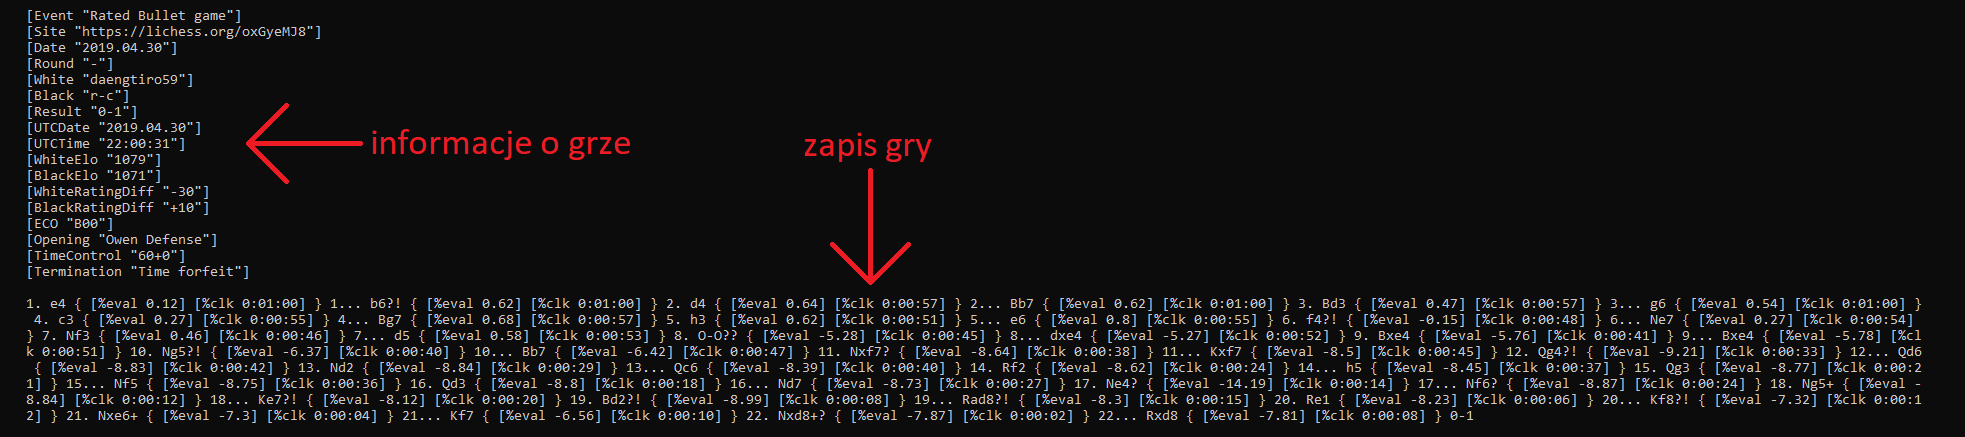
\includegraphics[width=\textwidth]{zapis_gry.png}
	\caption{Przykładowy zapis jednej partii zawierającej ocenę silnika Stockfish}
	\label{rys:zapis_gry} 
\end{figure}
Istotnym problemem związanym z danymi jest dokładność pozostałego czasu jedynie do sekund, co zaburza lekko ich istotę, szczególnie podczas analizy gier w krótszym formacie czasowym (jak np. ,,60+0''), gdzie ułamki sekundy są  znaczące. Dodatkowo ruch, który oznaczony został jako n sekund w rzeczywistości jest ruchem z przedziału obustronnie otwartego (n-1,n+1) sekund. Przy dużej liczbie danych nie ma to jednak większego znaczenia, ponieważ zgodnie z Prawem Wielkich Liczb można takie dane uśrednić do \textit{n} \textbf{cite???}. Jedynym problemem, który może się pojawić jest późniejsze sprawdzenie zgodności danych z rozkładem. 

\subsection{Odfiltrowanie danych}

Pierwszym krokiem potrzebnym do wykonania analizy jest odfiltrowanie danych.
Po rozdzieleniu pliku tekstowego na kolejne gry, pozostawione zostały jedynie te, które zostały wcześniej ocenione przez silnik oraz grane były w formacie ,,300+0'' lub ,,600+0''. Następnie przygotowany wcześniej program zbadał każdy ruch każdej gry i przypisał do niego następujące atrybuty:
\begin{itemize}
	\item game\_ID -- numer gry
	\item score -- ocena ruchu według silnika Stockfish
	\item delta\_time -- czas na wykonanie danego ruchu
	\item WhiteElo -- ranking białych
	\item BlackElo -- ranking czarnych
	\item TimeControl -- czas na wykonanie ruchów każdego z graczy w formacie  ,,sekundy + sekundy dodane za wykonanie ruchu''
	\item color -- gracz, wykonujący dany ruch
	\item move -- numer ruchu w danej partii
	\item result - wynik partii
\end{itemize}

Stworzona baza zawiera 17 524 012 posunięć ze 275 994 gier, co daje średnią 31,75 ruchu na grę (jeden ruch oznacza posunięcie białych i czarnych). Fragment bazy przedstawiony został na rysunku \ref{rys:baza_ruchow}. 
\begin{figure}[H]
	\centering
	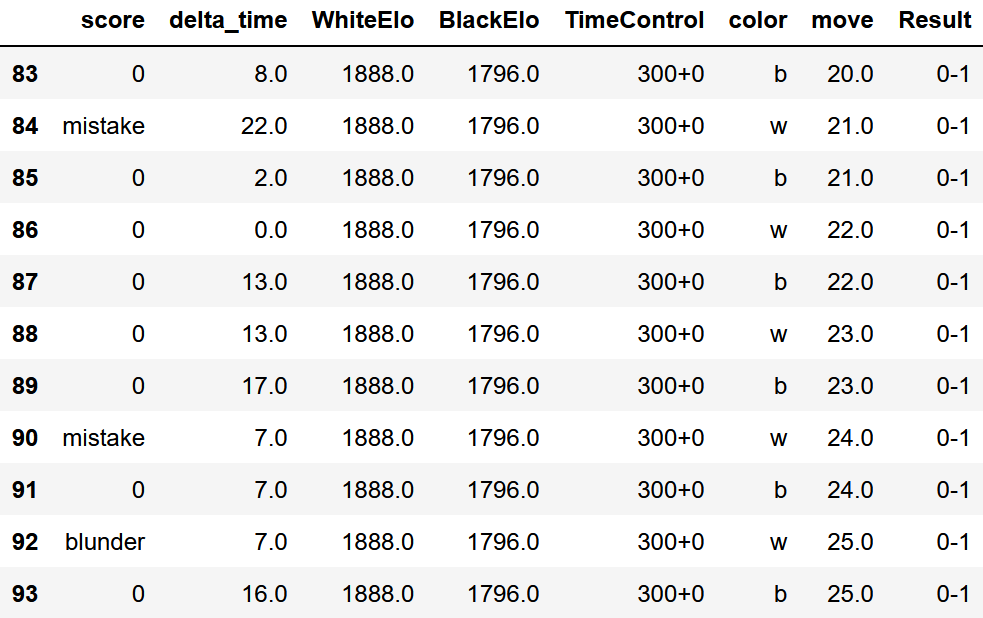
\includegraphics[width=\textwidth]{danee.png}
	\caption{Fragment bazy zawierającej ruchy z gier o formatach czasowych ,,300+0'' i ,,600+0''.}
	\label{rys:baza_ruchow}
\end{figure}




\section{Analiza problemu}

\subsection{Wstępny przegląd danych}



Pierwszym problemem, który zostanie poruszony jest zbadanie statystycznej zależności jakości wykonanego ruchu według oceny silnika Stockfish od czasu potrzebnego na jego wykonanie. W celu uzyskania bardziej precyzyjnych wyników pierwsze 4 ruchy (po 4 posunięcia białych i czarnych) nie będą brane pod uwagę. Są one elementem teorii otwarć szachowych [CITE??? \textbf{ref ISBN 0-19-280049-3}], w związku z czym wykonywane są zazwyczaj bardzo szybko i ze znikomą szansą popełnienia błędu, co może powodować zaburzenie danych. Dodatkowo na stronie Lichess.com pierwszy ruch obydwu zawodników zawsze zabiera 0 sekund.

Przy analizie z uwzględnieniem rankingu graczy, zastosowane będą podziały kwartylowe. Rozkład rankingu wraz z zaznaczonymi kwartylami pokazany jest na rysunku \ref{rys:rozklad_elo}. Jak widać zbiega on do rozkładu normalnego. Anomalia dla rankingu 1500 związana jest z tym, że jest to ranking przyznawany każdemu graczowi przy jego pierwszej rozgrywce na platformie.
\begin{figure}[H]
	\centering
	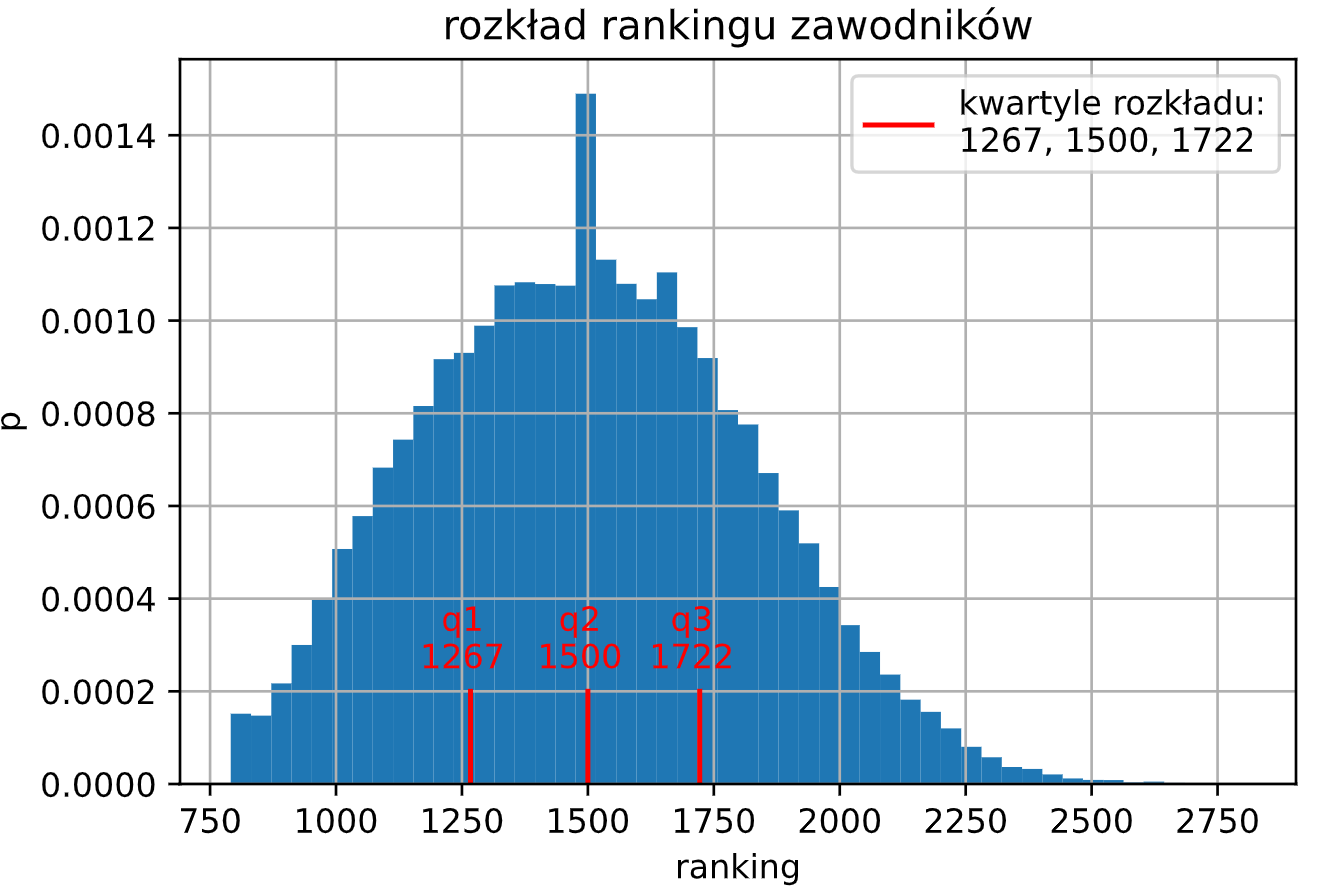
\includegraphics[width=\textwidth]{ranking.png}
	\caption{rozkład rankingu zawodników wraz z zaznaczonymi kwartylami}
	\label{rys:rozklad_elo}
\end{figure}
W późniejszej części pracy pojawią się wykresy i analizy, w których dziedziną będzie numer wykonywanego ruchu. W związku z bardzo małą liczbą danych dla późniejszych ruchów, ich analiza jest zaburzona i niewiarygodna. Dlatego analizowane będą jedynie ruchy z indeksem poniżej 59, jako, że wynik 95\% gier pojawia się maksymalnie w 58 ruchach. Rozkład długości gier z bazy danych, który obrazuje przedstawioną sytuację zamieszczony jest na rysunku \ref{rys:dlugosc_gier}.

\begin{figure}[H]
	\centering
	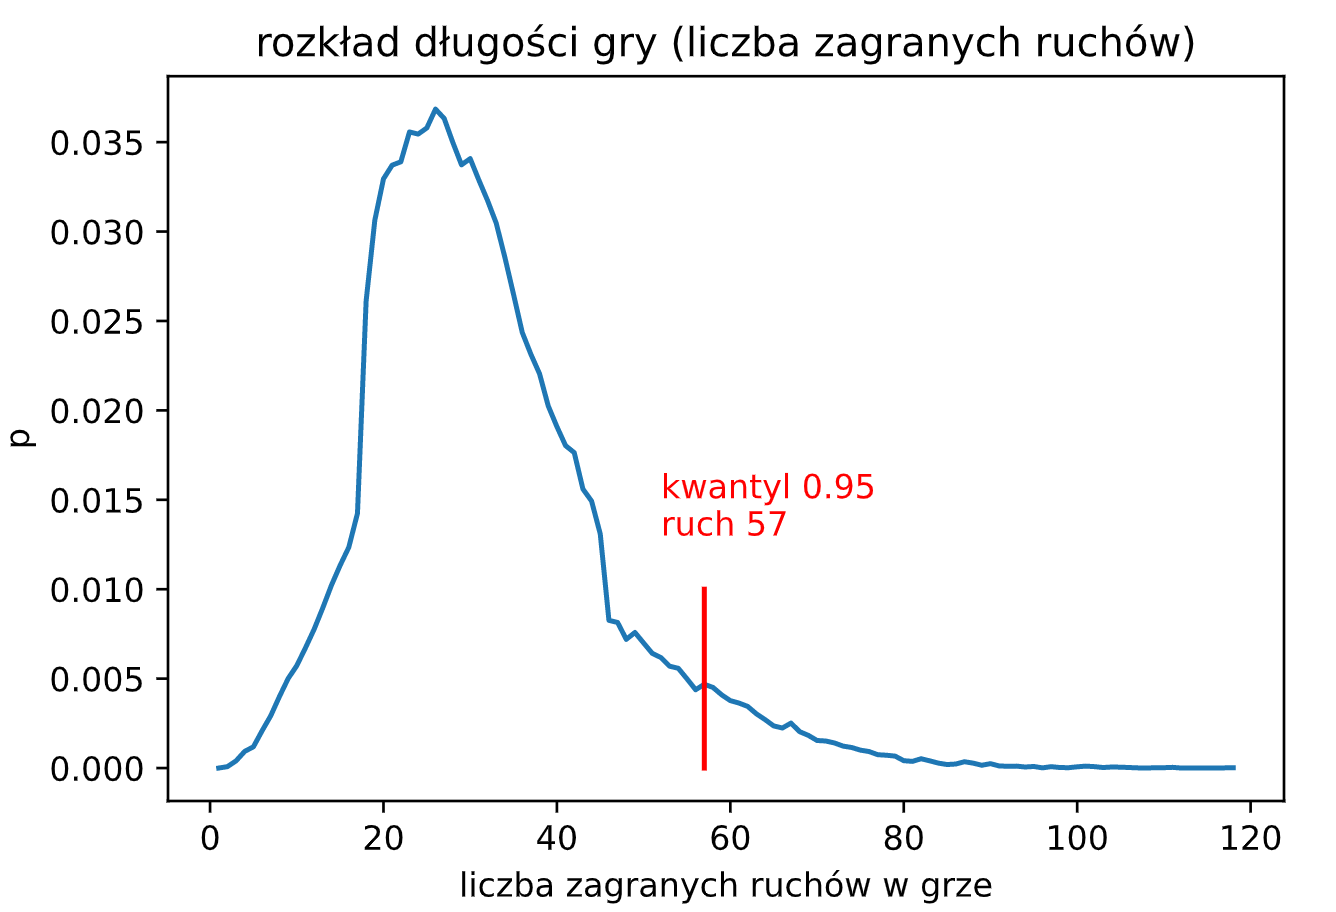
\includegraphics[width=\textwidth]{dlugosc_gry.png}
	\caption{rozkład długości gier wraz z zaznaczonym kwantylem rzędu 0.95,  dla gier z formatu 300+0 oraz 600+0.}
	\label{rys:dlugosc_gier}
\end{figure}


\subsection{Zależność między indeksem ruchu, a poświęconym czasem}


Na początku tej części trzeba ustalić pewne założenia dotyczące zestawu danych. W pojedynczej grze szachowej często występuje sytuacja, w której gracz długo myśli nad konkretnym posunięciem, rozpatrując możliwe następujące po nim sekwencje. W określonych okolicznościach, takich sekwencji jest na tyle mało, że każdy z graczy ma przez kilka kolejnych ruchów tylko jedno nieprzegrywające, łatwe do znalezienia posunięcie. Czas na wykonanie takich ruchów jest więc od siebie w pewien sposób zależny, jednakże sytuacje takie pojawiają się na bardzo nieoczekiwanie i przez mnogość zmiennych są trudne do znalezienia i uwzględnienia. Dlatego w celu ułatwienia analizy, w dalszych rozważaniach następujące po sobie ruchy będą uznawane za niezależne względem siebie.
\begin{figure}[H]
	\centering
	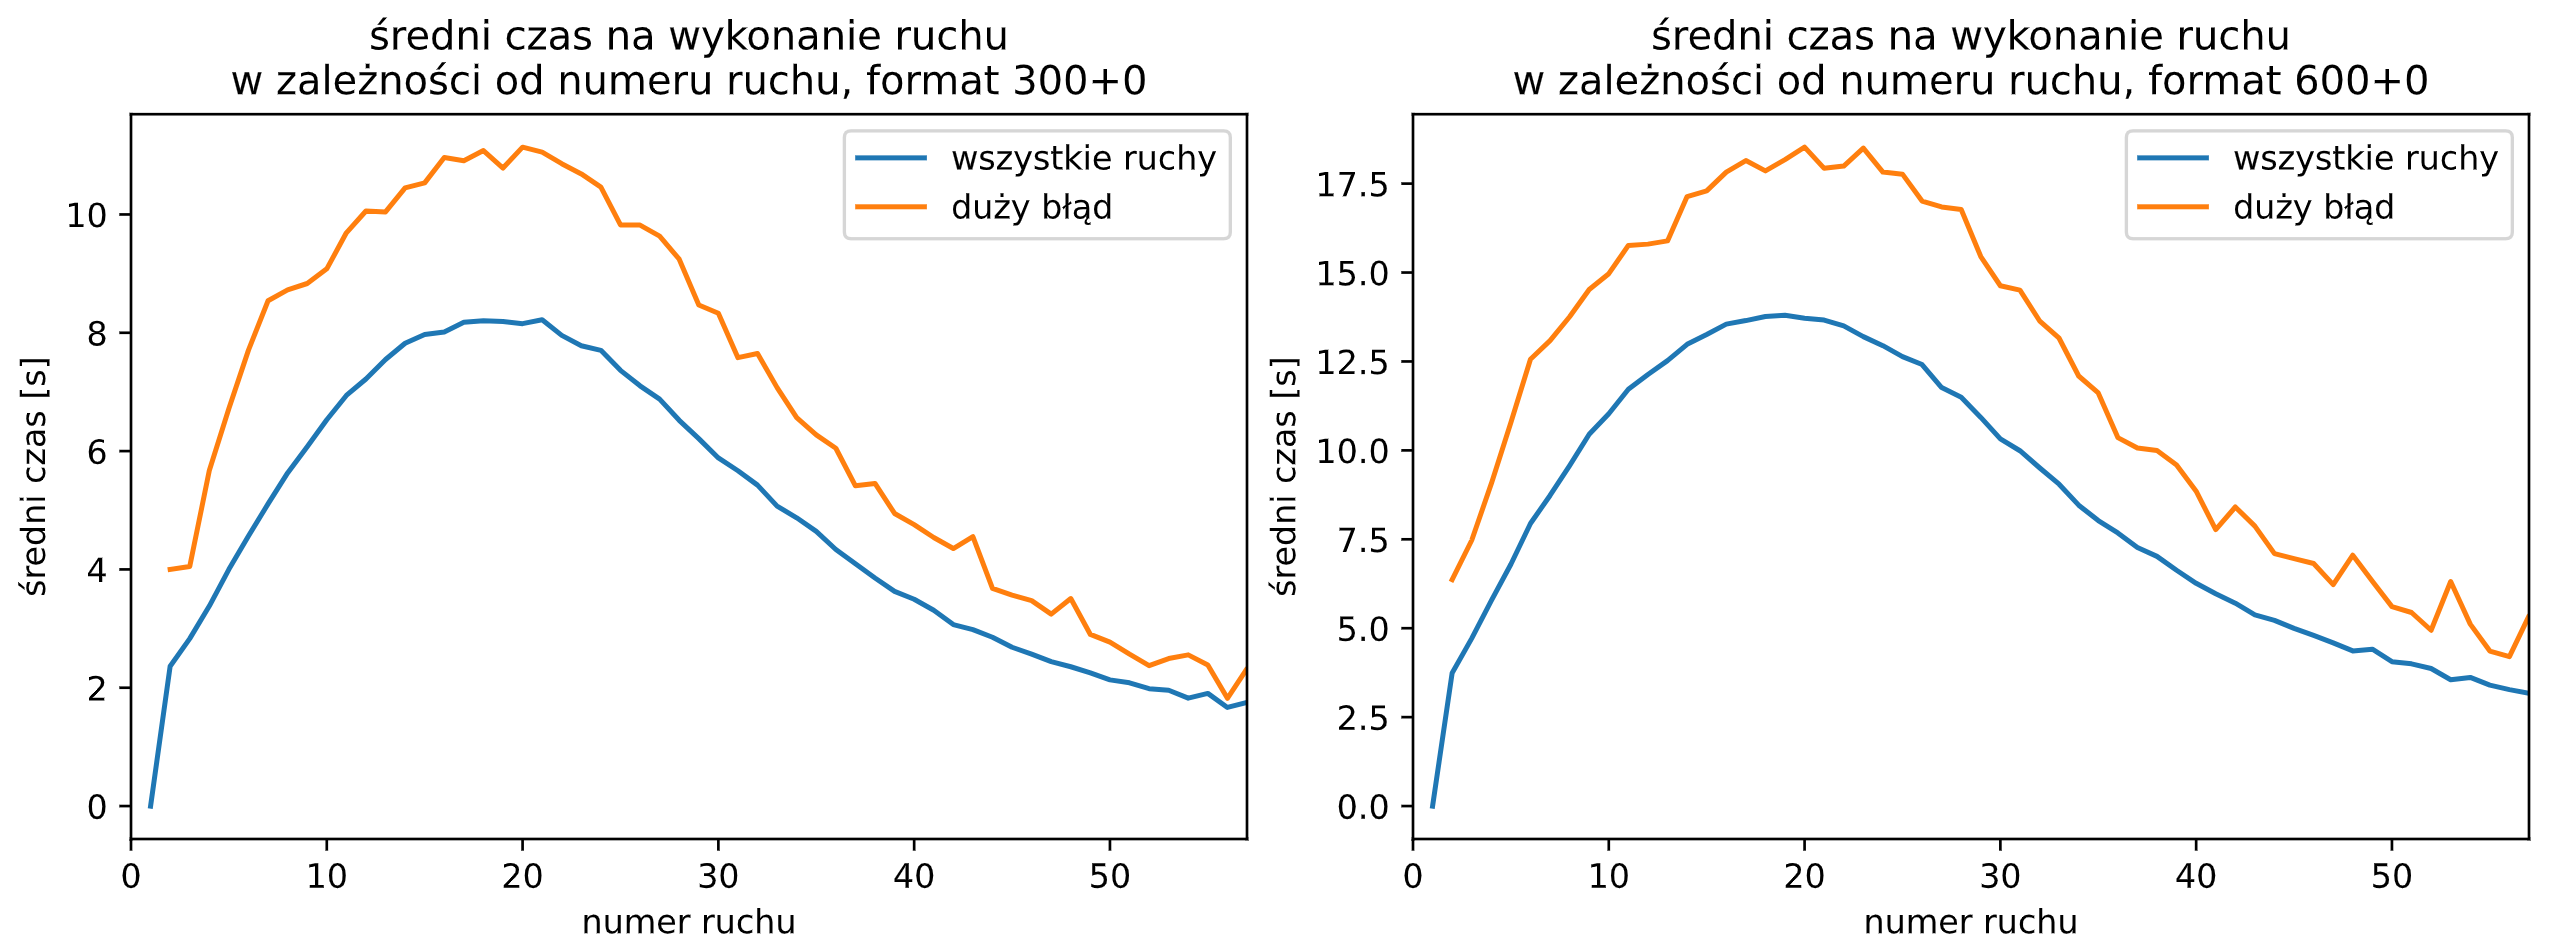
\includegraphics[width=\textwidth]{sr_czas_na_ruch.png}
	\caption{Średni czas na wykonanie ruchu dla analizowanych formatów czasowych wraz z zaznaczonym rozstępem międzykwartylowym. Osobno wszystkie ruchy i ruchy oznaczone przez silnik jako ,,duży błąd''.}
	\label{rys:sr_czas_na_ruch}
\end{figure}

Pierwszym elementem analizy, który pozwoli na określenie wstępnej różnicy między ruchami oznaczonymi jako ,,duży błąd'', a zbiorem wszystkich ruchów jest sprawdzenie zależności między indeksem ruchu, a średnim czasem na jego wykonanie dla obydwu zbiorów. Intuicja wskazuje, że błąd popełniamy poświęcając mniej czasu na ruch. Jak widać na rysunku \ref{rys:sr_czas_na_ruch}, dla każdego analizowanego ruchu, ruch oznaczony jako błędny zajął statystycznie więcej czasu - zarówno dla formatu 300+0 jak i 600+0, co przeczy intuicji. 
Przyczyną tego może być zaliczanie do zbioru wszystkich ruchów posunięć oczywistych, zajmujących niewielką ilość czasu, następujących dla pozycji, w której gracze na każdym poziomie zaawansowania rzadko kiedy popełniają błędy.
Kolejną przyczyną takiego stanu rzeczy może być oczywista zależność skomplikowania pozycji od szansy na popełnienie błędu. W trudnych sytuacjach na szachownicy błędów pojawia się po prostu więcej, a trudnych sytuacji najwięcej jest w środkowej części partii, przez mnogość figur i możliwych legalnych ruchów. Trudno też znaleźć takie pozycje, ponieważ zależą one od przyjętej miary, o czym pisze D. H. Holding w swojej pracy zatytuowanej \textit{,,Evaluation of Chess Positions''} \textbf{CITE Holding, D. H. (1979). The Evaluation of Chess Positions. Simulation \& Games, 10(2), 207–221. doi:10.1177/104687817901000205}  Dlatego też, co widoczne jest na wykresie, w środkowej części gry, posunięcia zajmują najwięcej czasu.

Po oznaczeniu \textit{D} jako zmienną określającą skomplikowanie pozycji, \textit{T} - zmienną określającą czas na wykonanie ruchu w danej pozycji, \textit{B} - zdarzenie polegające na tym, że posunięcie jest błędne i przy założeniu, że \textit{T} jest silnie dodatnio skorelowane z \textit{R}, według prawdopodobieństwa otrzymujemy \textbf{SPRAWDZIĆ TO JESZCZE!}:
\begin{equation}
	P(B|D>d_0) > P(B|D\leq d_0) \rightarrow P(B|T>t_0) > P(B|T\leq t_0)
\end{equation}
gdzie $d_0$ i $t_0$ określają punkty, od których według wybranej miary można określić, że pozycja jest skomplikowana ($D>d_0$) i czas na wykonanie posunięcia jest długi ($T>t_0$).


Może to tłumaczyć wyższą średnią czasu na wykonanie błędnego posunięcia w porównaniu do zbioru wszystkich posunięć.
\begin{figure}[H]
	\centering
	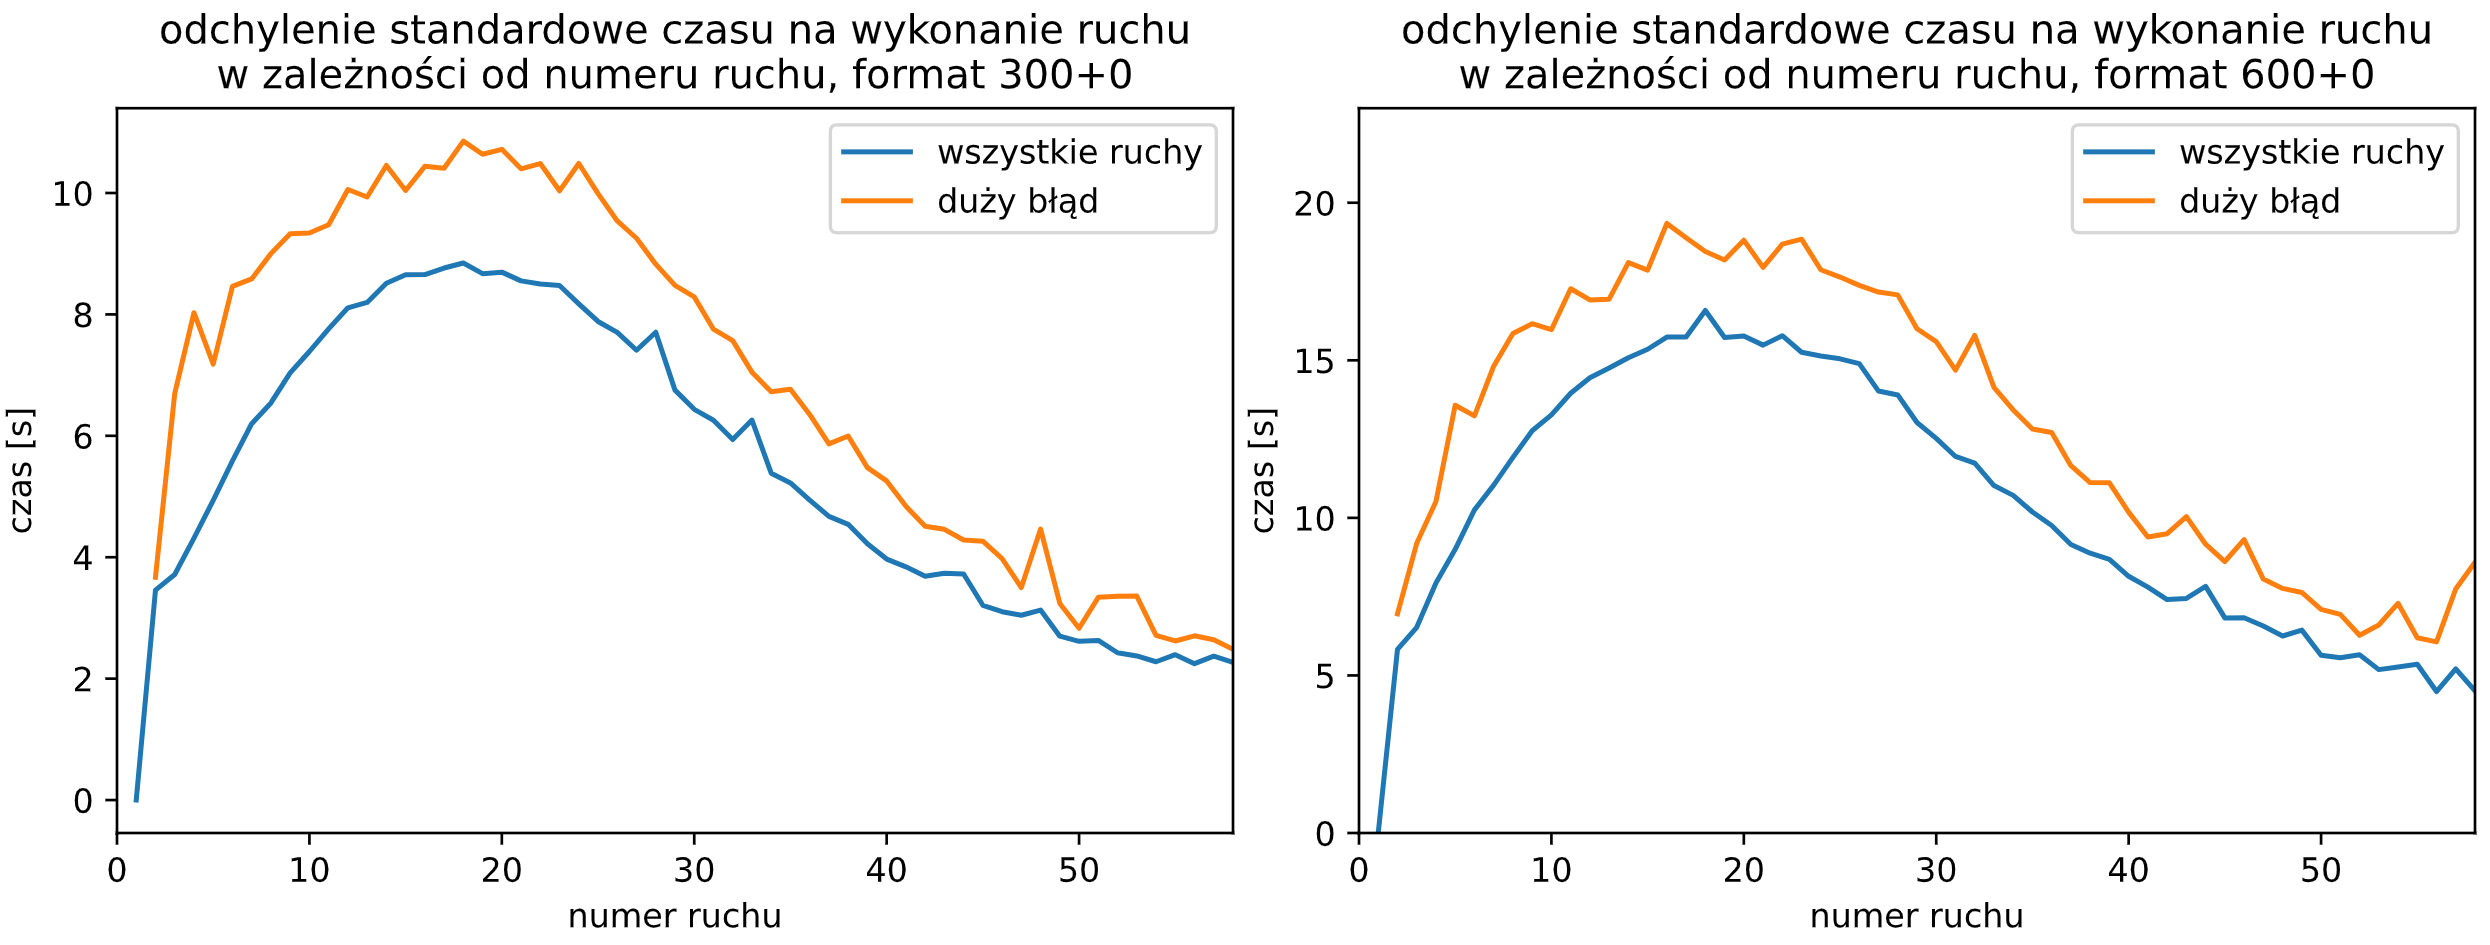
\includegraphics[width=\textwidth]{std_czas_na_ruch.png}
	\caption{Odchylenie standardowe czasu na wykonanie ruchu dla analizowanych formatów czasowych. Osobno wszystkie ruchy i ruchy oznaczone przez silnik jako ,,duży błąd''.}
	\label{rys:std_czas_na_ruch}
\end{figure}

Badając w dalszym ciągu wykresy na rysunku \ref{rys:sr_czas_na_ruch} można zauważyć, że dla obydwu zbiorów posunięć początkowo niska średnia osiąga swój szczyt w okolicach dwudziestego ruchu, by później stopniowo się zmniejszać. Ma to związek z tym, że początkowe posunięcia są elementem teorii szachowej. Duża część graczy nauczyła się kilku, kilkunastu, bądź w przypadku gry na najwyższym poziomie - nawet ponad dwudziestu pierwszych ruchów niektórych otwarć. W związku z tym początkowe ruchy grane są relatywnie szybko. Końcowe posunięcia natomiast nie mogą zająć zbyt dużo czasu, ponieważ jest go zazwyczaj zbyt mało na zegarze, by gracz mógł sobie na to pozwolić. Dlatego też od pewnego momentu, wraz ze wzrostem indeksu średni czas poświęcony na ruch zbiega do zera. Zaznaczone na rysunku rozstępy międzykwartylowe dla każdego ruchu wskazują na znacznie większą wariancję czasu na wykonanie błędnego ruchu porównując do zbioru wszystkich ruchów. Potwierdza to rysunek \ref{rys:std_czas_na_ruch} pokazujący odchylenie standardowe dla kolejnych ruchów. 
\begin{figure}[H]
	\centering
	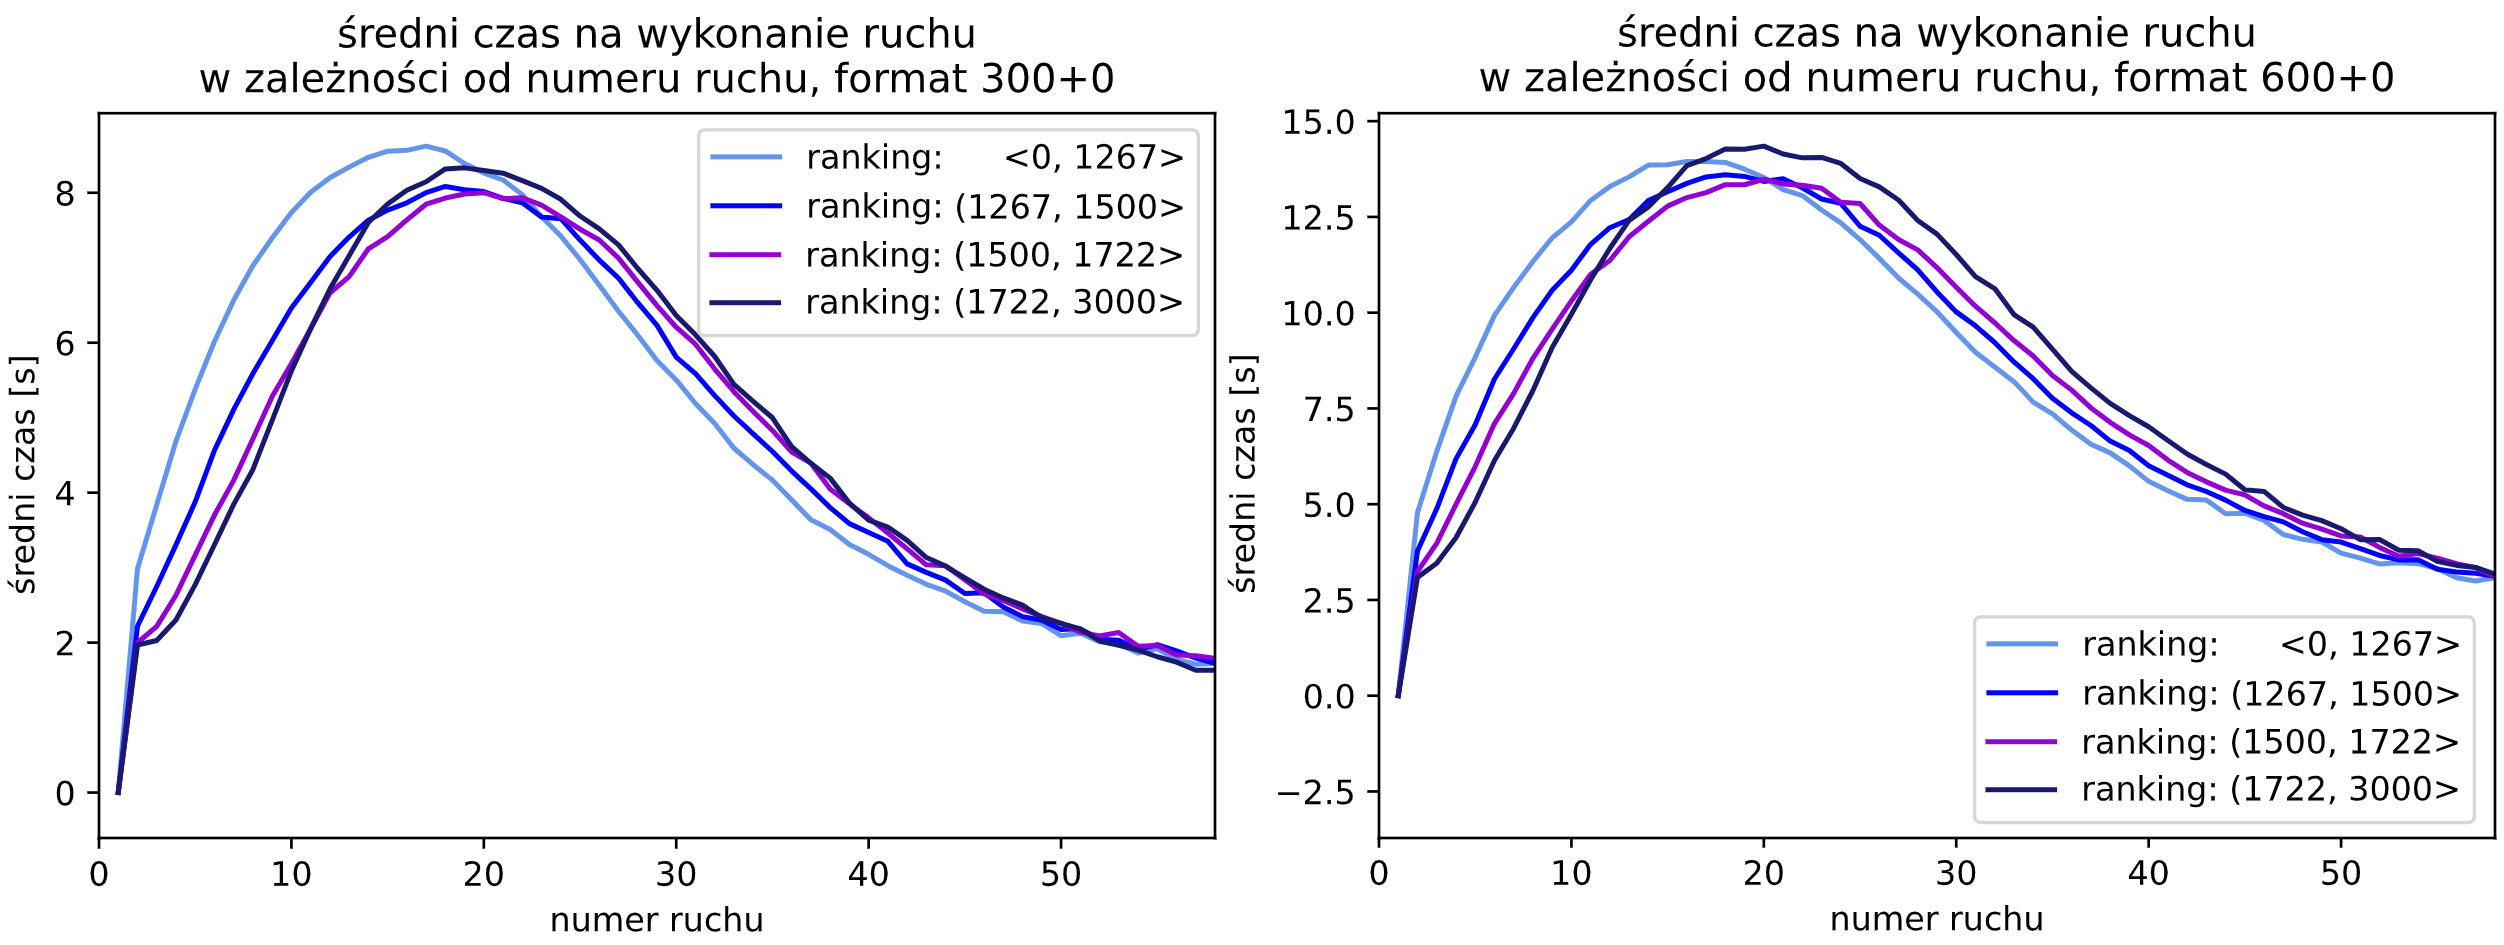
\includegraphics[width=\textwidth]{sr_czas_na_ruch_ELO_1.png}
	\caption{Średni czas na wykonanie ruchu dla dla graczy z różnych przedziałów rankingowych. Wszystkie posunięcia.}
	\label{rys:sr_czas_na_ruch_ELO_1}
\end{figure}

Rysunki \ref{rys:sr_czas_na_ruch_ELO_1} i \ref{rys:sr_czas_na_ruch_ELO_2} wprowadzają do rozważań różnicę między średnim czasem na wykonanie ruchu dla graczy z poszczególnych przedziałów rankingowych. Można zauważyć, że zarówno w przypadku zbioru wszystkich ruchów (rysunek \ref{rys:sr_czas_na_ruch_ELO_1}) jak i pozdbioru ruchów błędnych (rysunek \ref{rys:sr_czas_na_ruch_ELO_2}), słabsi gracze mają tendencję do dłuższych rozważań nad początkowymi ruchami. Wraz ze wzrostem rankingu wydłuża się średni czas na wykonanie ruchu dla ruchów z indeksem od 20 do 30 - czyli tych, gdzie średnia jest najwyższa. Przy końcowych posunięciach, posunięcia zajmują podobną ilość czasu dla wszystkich rankingów. Warto zwrócić uwagę, że odsetek 25\% najniżej notowanych graczy przez zbyt długie początkowe ruchy zmuszona jest ruszać się szybciej w późniejszych posunięciach. Szczególnie widoczne jest to na pierwszym wykresie rysunku \ref{rys:sr_czas_na_ruch_ELO_2}. 

\begin{figure}[H]
	\centering
	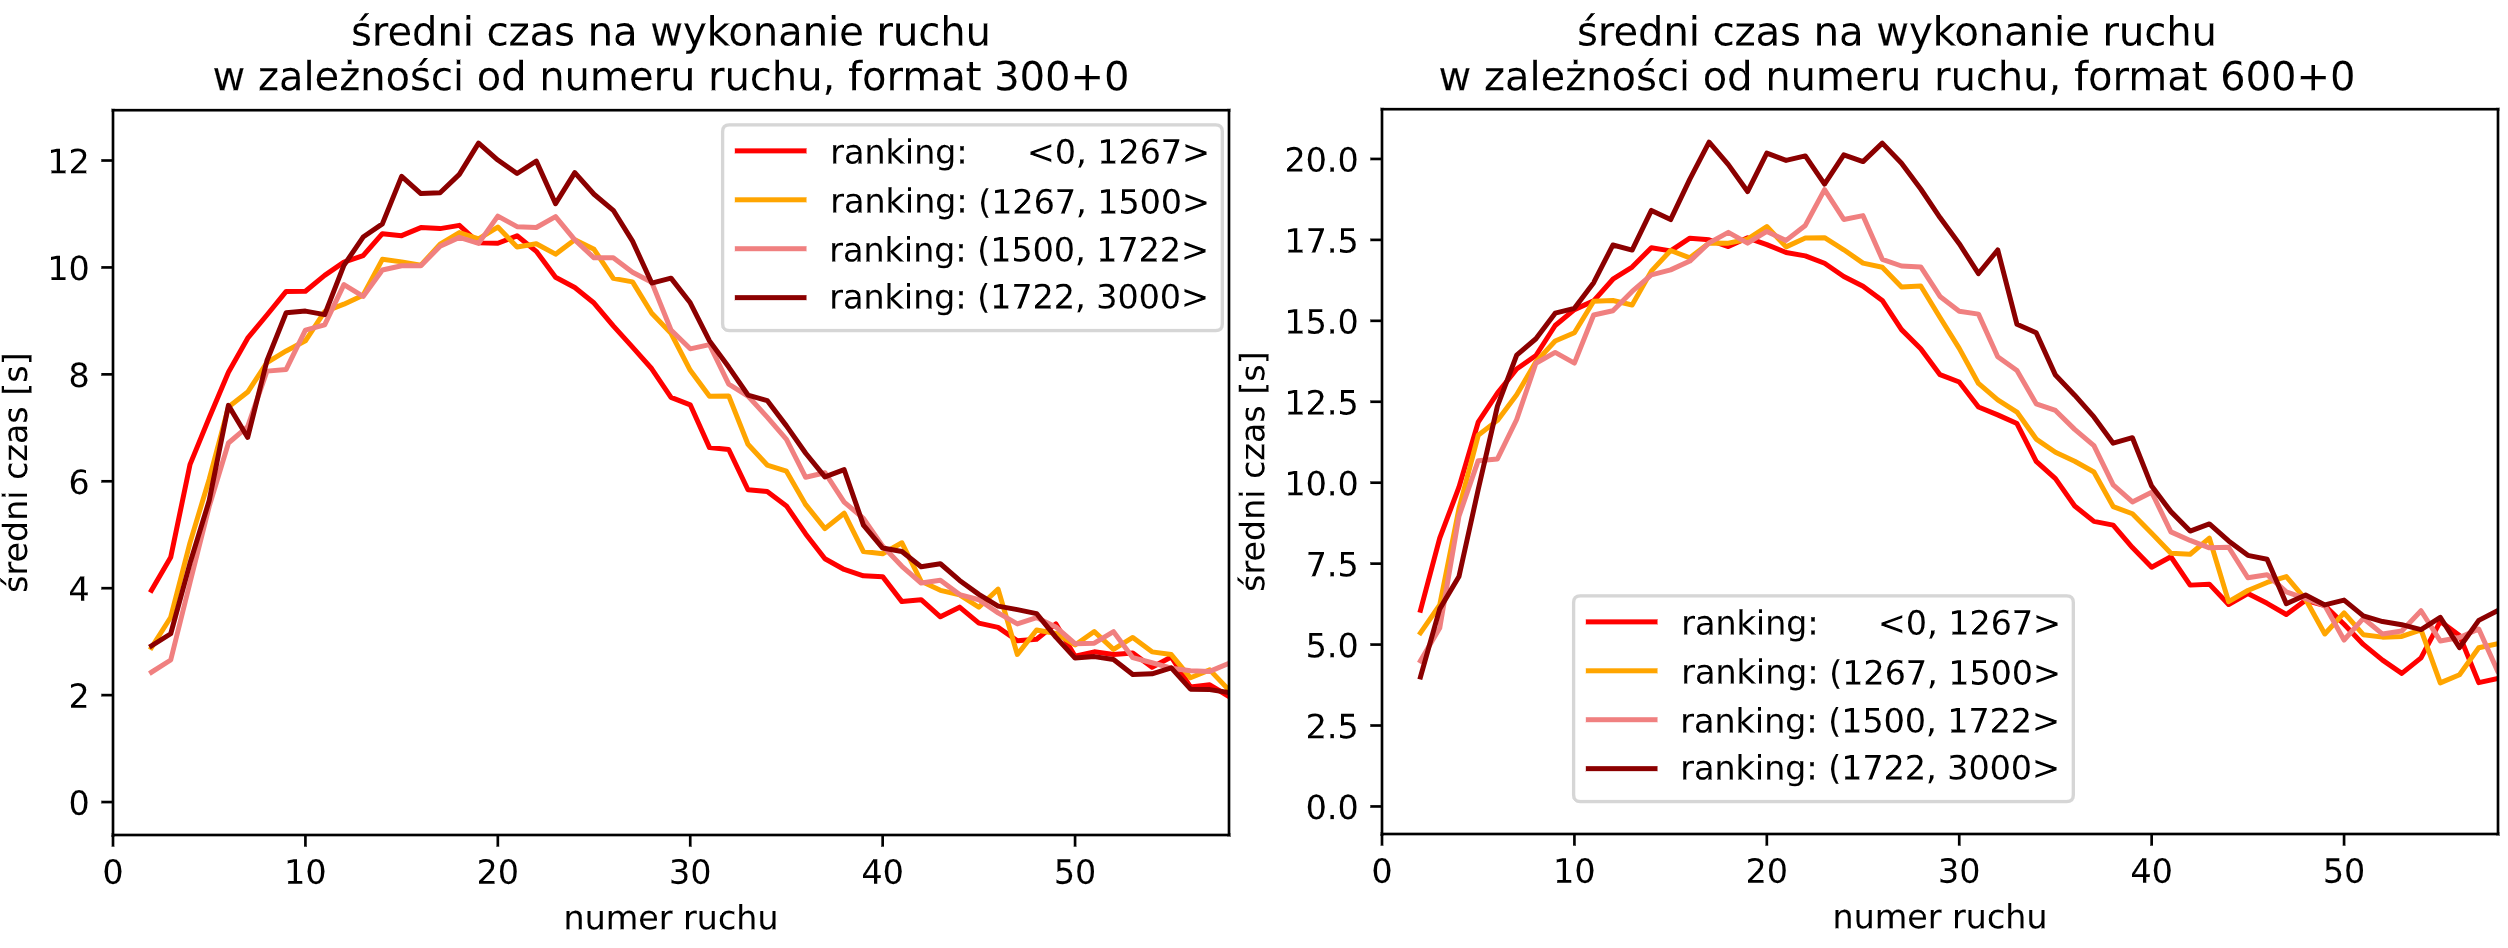
\includegraphics[width=\textwidth]{sr_czas_na_ruch_ELO_2.png}
	\caption{Średni czas na wykonanie ruchu dla dla graczy z różnych przedziałów rankingowych. Posunięcia oznaczone przez silnik jako ,,duży błąd''.}
	\label{rys:sr_czas_na_ruch_ELO_2}
\end{figure}
Niezależnie od rankingu, średnia poświęconego czasu dla posunięć oznaczonych przez silnik jako ,,duży błąd'' jest w każdym momencie wyższa niż dla zbioru wszystkich ruchów. 
Warto również zauważyć, że wykresy dla obydwu formatów czasowych wyglądają podobnie. 

By móc przeanalizować zależność między rozgrywanym formatem, a wzrostem średniego czasu poświęconego na ruch, powstał wykres umieszczony na rysunku \ref{rys:stosunek_sr_czas}. Dopasowane metodą najmniejszych kwadratów \textbf{OPISANĄ W ROZDZIALE TEORIA2???} proste regresji \textbf{DODAĆ COŚ O RESIDUACH I ODCHYLENIACH?, można zrobić też proste ze wszystkich danych,a nie ze średniej} obrazują różnice w zachowanych trendach. Czas w formacie 600+0 jest dokładnie 2 razy dłuższy niż w formacie 300+0, jednak średni czas na wykonanie ruchu jest w pierwszym przypadku około 1,7 raza wyższy. Wartość stosunku jednak nie jest stała i wzrasta wraz z indeksem ruchu. Dla zbioru wszystkich posunięć dopasowana prosta regresji wskazuje na stosunek około 1,65 dla tych początkowych, do 1,85 przy końcowych. Znacznie większa rozpiętość w stosunku widoczna jest dla posunięć oznaczonych jako ,,duży błąd''. Stosunek wynosi około 1,55 dla początkowych wartości i powyżej 2 dla ruchów z indeksem powyżej 55. Warto zauważyć, że dla obu zbiorów w formacie 600+0 gracze nie są zmuszeni do podejmowania decyzji pod dużą presją czasu. Szczególnie różnicę tę da się zauważyć dla ruchów błędnych, nad którymi gracz musi się statystycznie dłużej zastanowić (rysunek \ref{rys:sr_czas_na_ruch} na stronie \pageref{rys:sr_czas_na_ruch}). Gracz posiadając 2 razy więcej czasu w tym formacie i myśląc nad każdym ruchem średnio od 1.55 do 1.95 raza dłużej,  ma w każdym momencie gry do dyspozycji statystycznie większy ułamek początkowego czasu niż w przypadku gry w formacie 300+0. Zestawienie pozostałego czasu pokazane jest na pierwszym wykresie na rysunku rysunku \ref{rys:pozostaly_czas}. Widać dość sporą różnicę w średnim pozostałym czasie narastającą podczas przebiegu gry. Drugi wykres zamieszczony na rysunku ukazuje różnicę w prawdopodobieństwie popełnienia błędu w konkretnym ruchu dla obu formatów. Warto zauważyć, że mimo znacznie większego czasu do dyspozycji w przypadku formatu ,,600+0'', do 20 ruchu szansa na błąd jest niemalże identyczna jak w przypadku formatu ,,300+0'' -- Krzywe odbiegają od siebie nieznacznie. W okolicach od 20 do 40 ruchu, szansa na popełnienie błędu w formacie ,,300+0'' jest około 5-10\% większa. Dobrze jest w tym miejscu dodać, że jest to przedział, w którym błędów występuje najwięcej.

\textbf{jakiś bayes później? }

\begin{figure}[H]
	\centering
	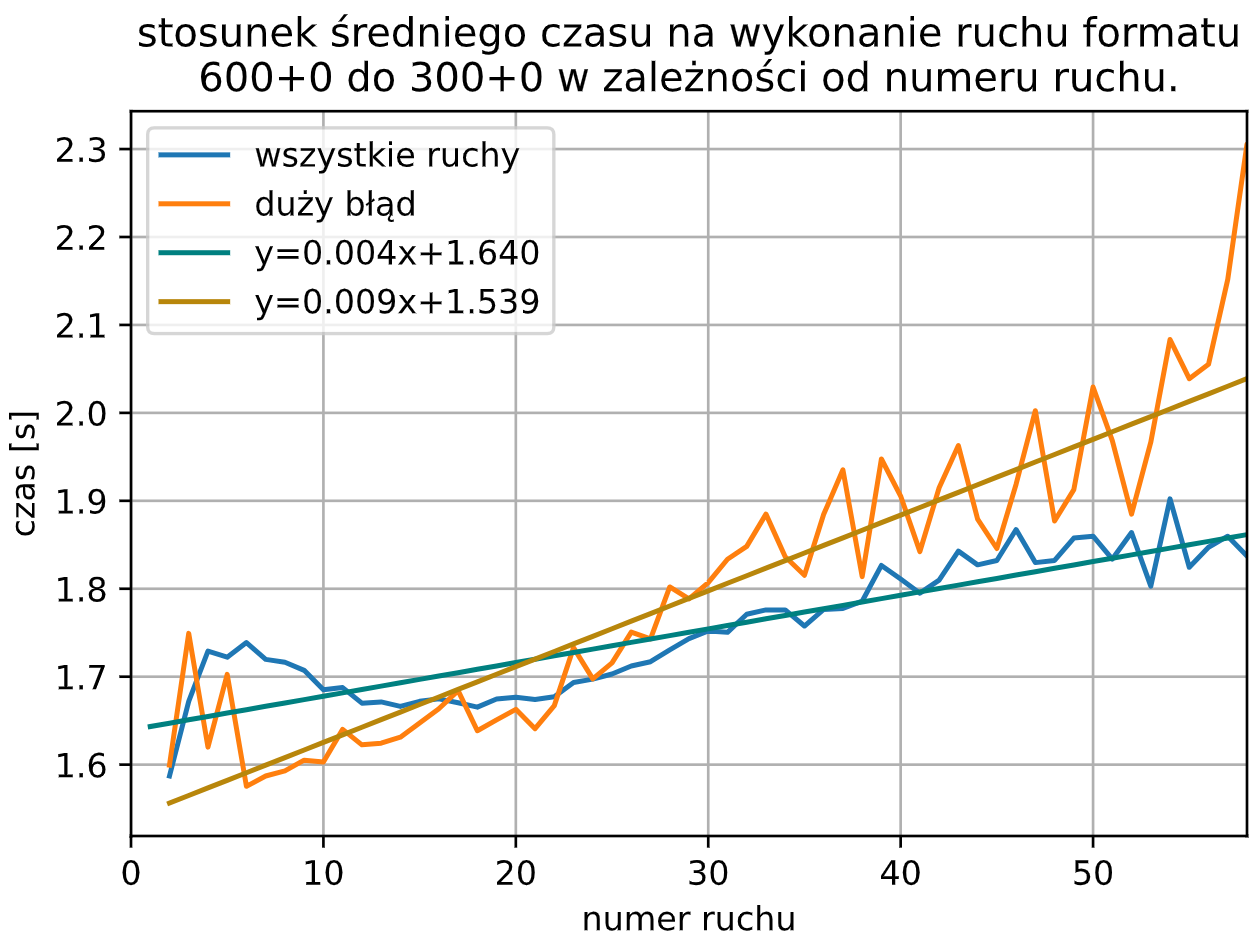
\includegraphics[width=\textwidth]{stosunek_sr_czas.png}
	\caption{Stosunek średniego czasu na wykonanie ruchu w formacie 600+0 do czasu w formacie 300+0. Zaznaczone proste regresji obrazujące trend.}
	\label{rys:stosunek_sr_czas}
\end{figure}
\begin{figure}[H]
	\centering
	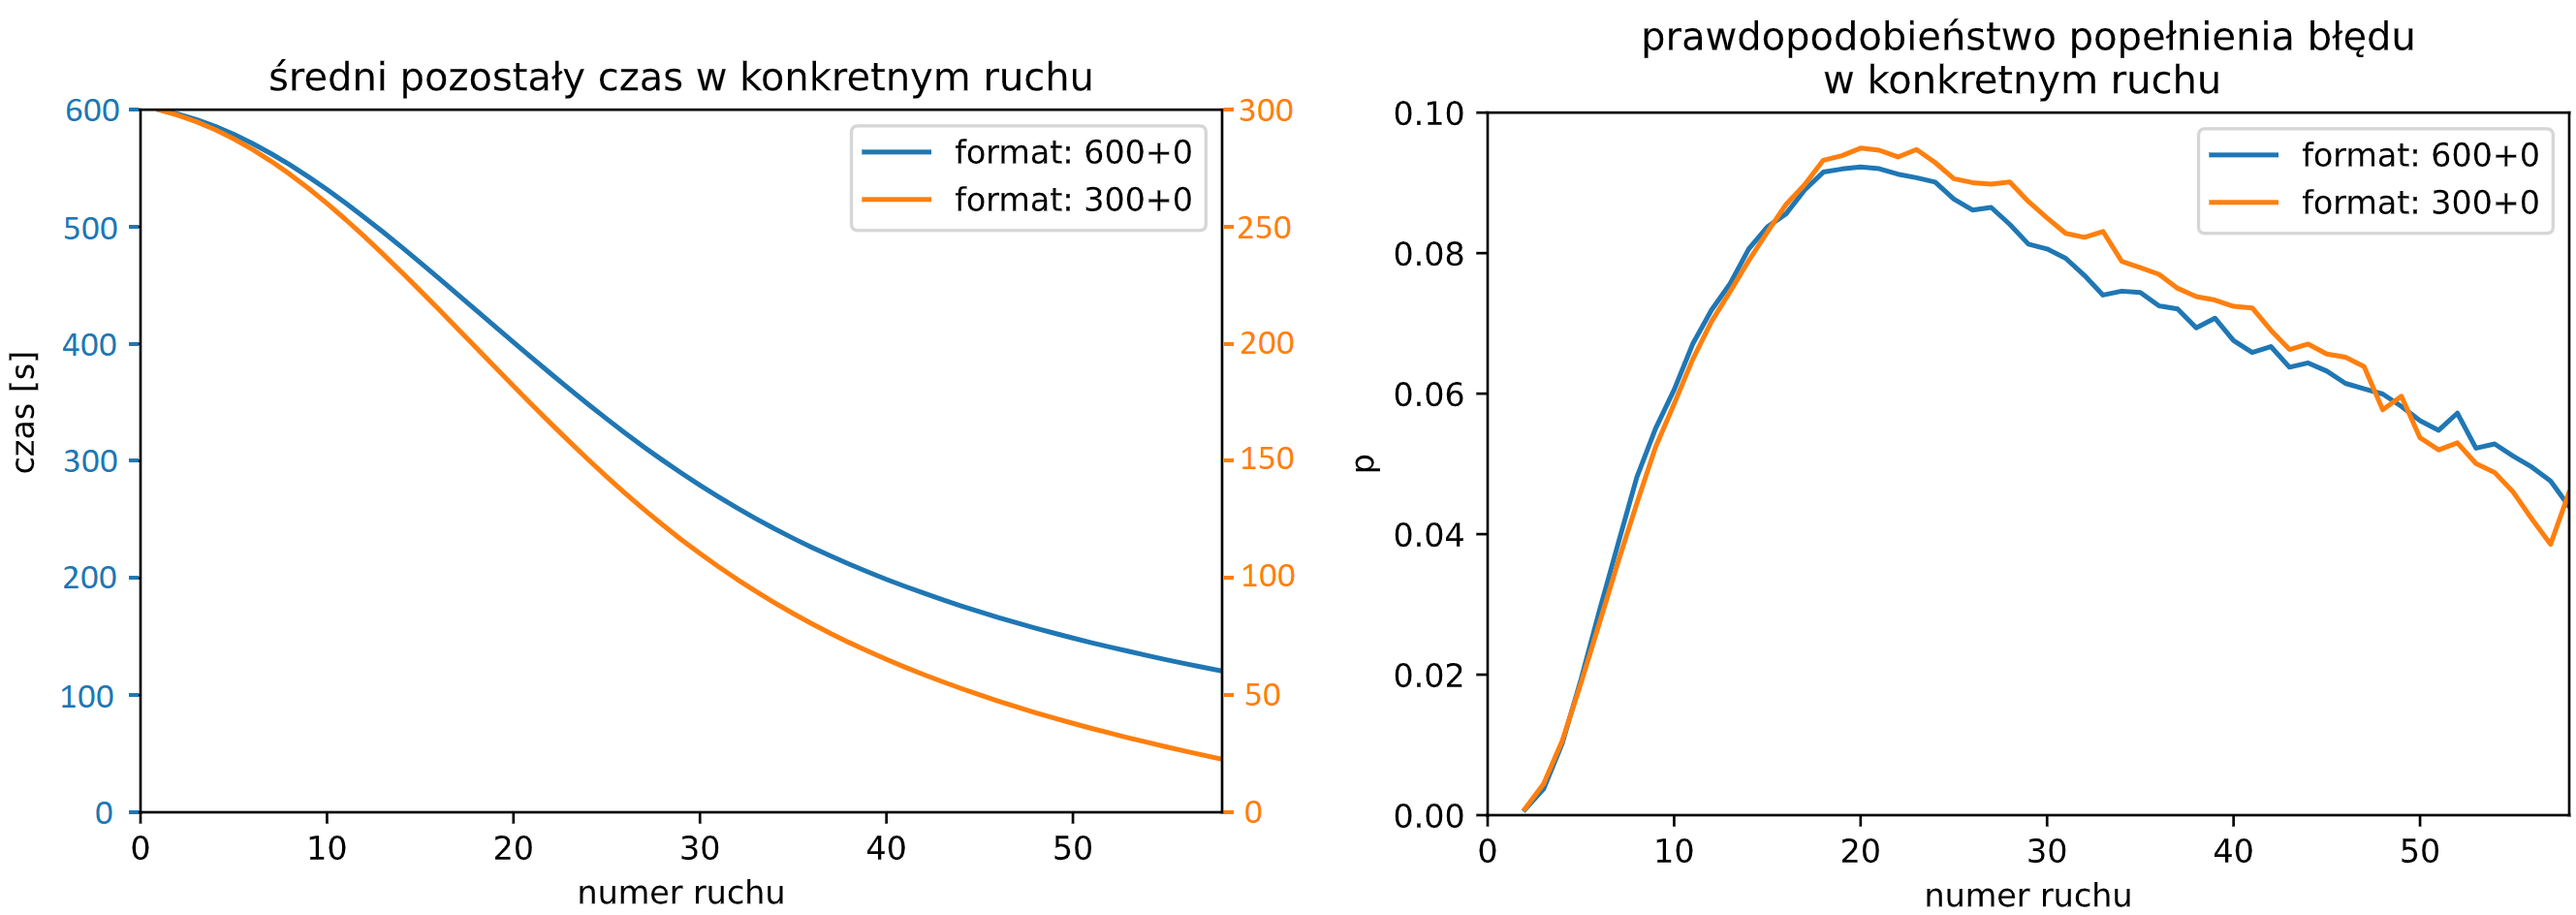
\includegraphics[width=\textwidth]{pozostaly_czas.png}
	\caption{
		Pierwszy wykres -- zestawienie średniego pozostałego czasu w formatach 600+0 oraz 300+0. W celu lepszego porównania zastosowane osobne osie dla każdego formatu. Drugi wykres -- empiryczne prawdopodobieństwo popełnienia błędu w konkretnym ruchu.}
	\label{rys:pozostaly_czas}
\end{figure}
\begin{figure}[H]
	\centering
	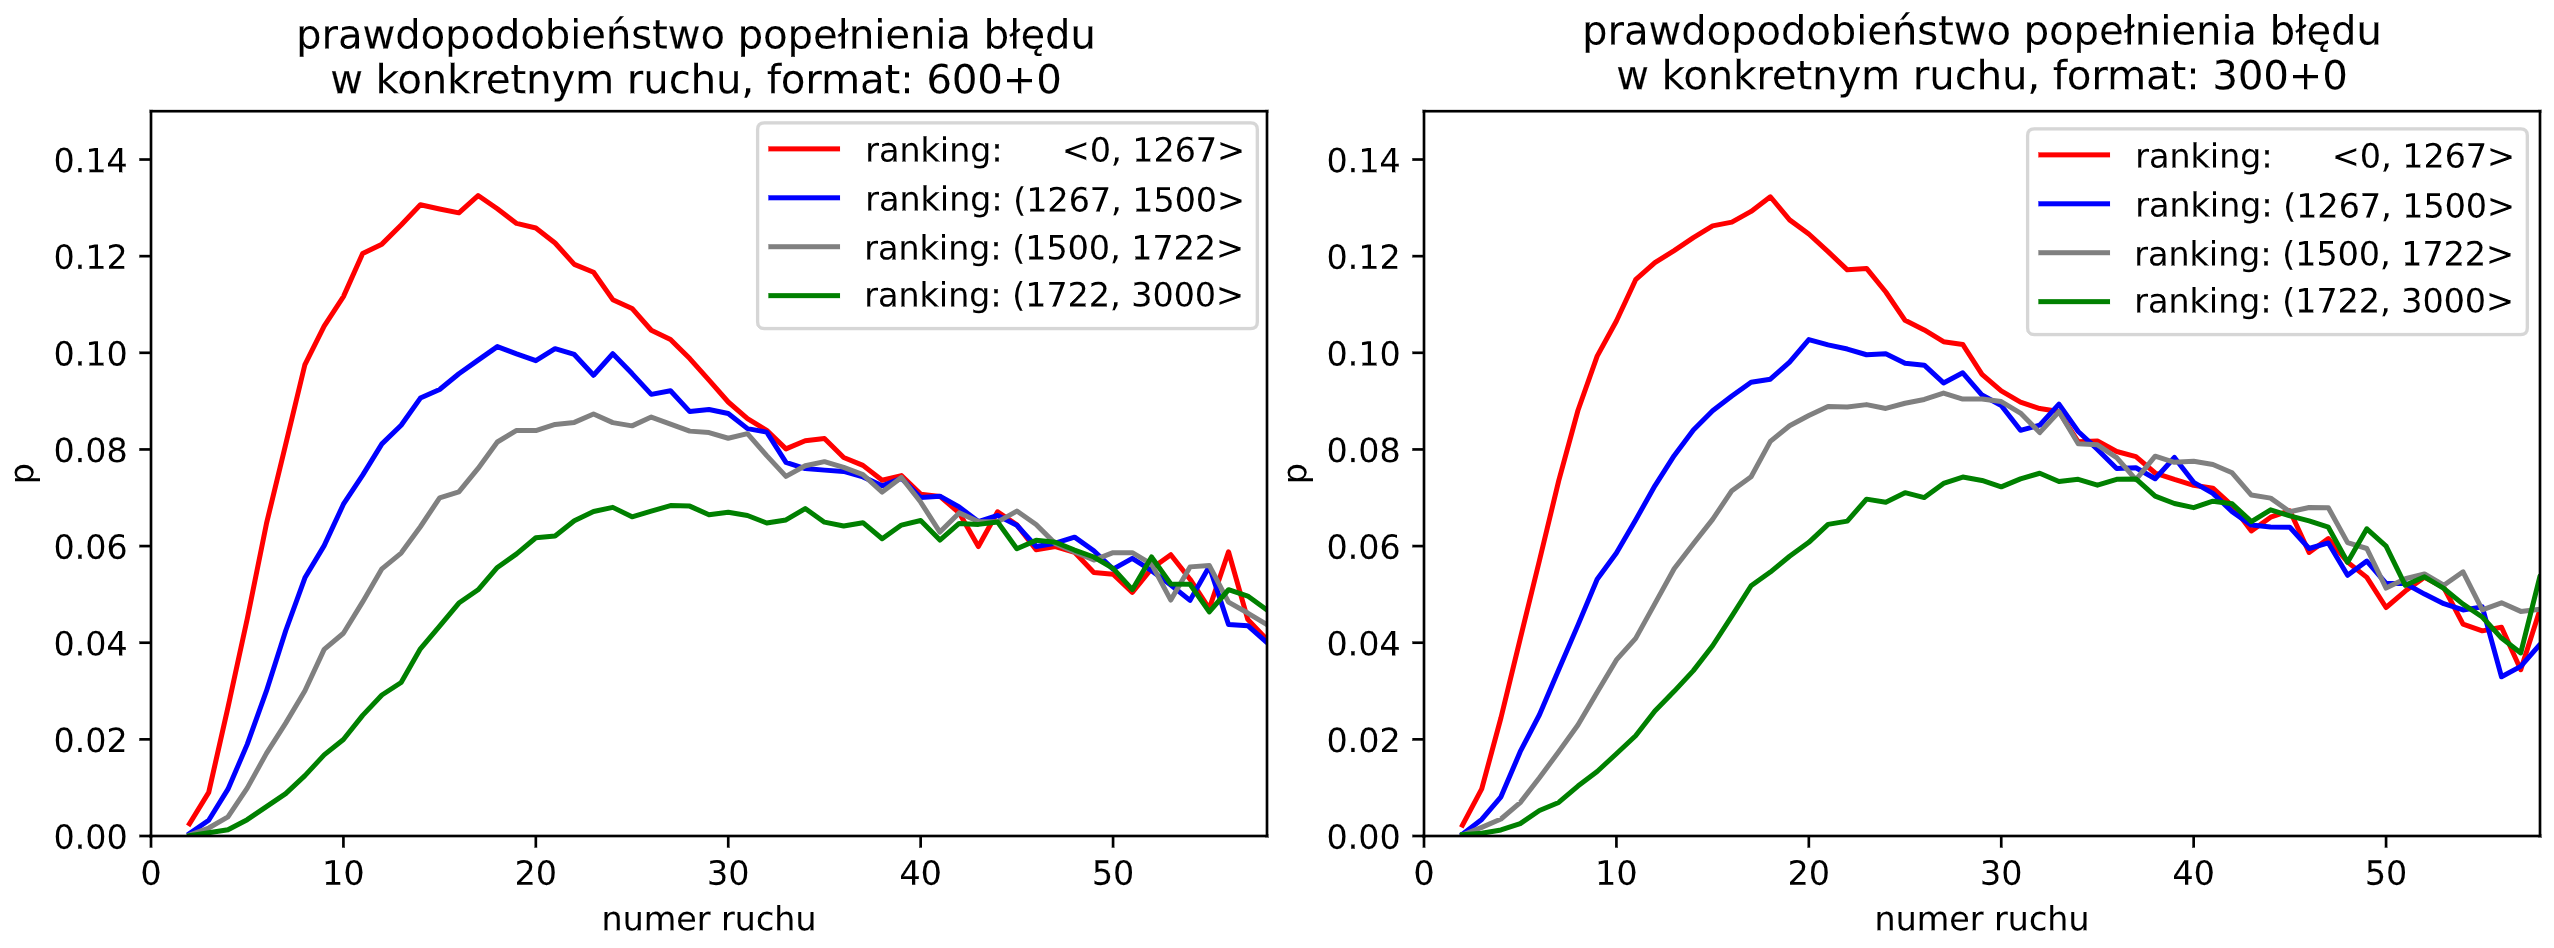
\includegraphics[width=\textwidth]{prawd_blad_ELO.png}
	\caption{
		blblalsdlasdlasldlad.}
	\label{rys:prawd_blad_ELO}
\end{figure}
Różnica w prawdopodobieństwie popełnienia błędu pomiędzy poszczególnymi formatami nie jest tak duża jak ta pomiędzy rankingiem graczy. Na rysunku \ref{rys:prawd_blad_ELO} można zauważyć, że dla zarówno dla formatu ,,600+0'' jak i ,,300+0'' słabsi gracze mają tendencję do popełniania większej liczby błędów w początkowej fazie gry, niż ich wyżej notowani koledzy. Statystycznie, będąc w grupie 25\% najniżej notowanych graczy ma się około 6 razy większe prawdopodobieństwo na popełnienie błędu w 10 posunięciu, niż osoba z grupy 25\% najwyżej notowanych graczy. Format gry ma na to niewielki wpływ. Można wysunąć wniosek, że w przypadku gry pomiędzy dwoma takimi zawodnikami, dwukrotnie zwiększenie czasu niżej notowanego gracza z 5 do 10 minut będzie miało minimalny wpływ na finalny wynik gry (przy założeniu, że liczba ,,dużych błędów'' jest mocno skorelowana z wynikiem gry). krzywe zaczynają do siebie zbiegać od okolic 20 ruchu, by stać się praktycznie nierozróżnialne w okolicach 40 ruchu.

Wykres zależności prawdopodobieństwa od ruchu jest tym bardziej ,,spłaszczony'' im wyższa jest notacja elo zawodników. Brak szybkiego wzrostu dla początkowych posunięć sprawia, że statystyczne prawdopodobieństwo popełnienia ,,dużego błędu'' w pierwszych 10 ruchach niesamowicie różni się dla poszczególnych grup rankingowych. Tabela \ref{tab:blad_w_n_ruchach} przedstawia różnicę w szansie na popełnienie przynajmniej jednego błędu w pierwszych 10, 20 i 30 ruchach dla graczy z określonych przedziałów rankingowych i gier w określonym formacie. Przykładowo, dla osoby z grupy 25\% najniżej notowanych graczy grającej w formacie ,,600+0'', szansa na popełnienie błędu w 10 pierwszych ruchach wynosi aż 43,46\%, natomiast dla grupy 25\% najlepszych graczy jest to jedynie 6,76\%. Różnica ta zmniejsza się znacząco, gdy weźmie się pod uwagę większą liczbę pierwszych ruchów. Dla 20, jest to kolejno 85,50\% i 40,78\%, a dla 30 -- 95,32\% i 70,27\%. Wartości te wyglądają podobnie dla formatu 300+0.
\begin{table}[H]
	\caption{Szansa na popełnienie błędu w pierwszych \textit{n} ruchach dla gracza z określonego przedziału rankingowego z rozdzieleniem na formaty ,,600+0'' i ,,300+0''}
	\centering
	\begin{tabular}{|l|r|r|r|r|r|r|l}
		\cline{1-7}
		\textbf{\begin{tabular}[c]{@{}l@{}}\textit{n} pierwszych \\ ruchów\end{tabular}} & \multicolumn{2}{l|}{\textbf{n = 10}}                                      & \multicolumn{2}{l|}{\textbf{n = 20}}                                      & \multicolumn{2}{l|}{\textbf{n = 30}}                                      & \textbf{} \\ \cline{1-7}
		\textbf{centyl\hphantom{ } \textbackslash \hphantom{ } format}                                   & \multicolumn{1}{l|}{\textbf{600+0}} & \multicolumn{1}{l|}{\textbf{300+0}} & \multicolumn{1}{l|}{\textbf{600+0}} & \multicolumn{1}{l|}{\textbf{300+0}} & \multicolumn{1}{l|}{\textbf{600+0}} & \multicolumn{1}{l|}{\textbf{300+0}} &           \\ \cline{1-7}
		\textbf{0-25\%}                                                         & 43,36\%                             & 40,72\%                             & 85,50\%                             & 84,33\%                             & 95,32\%                             & 94,96\%                             &           \\ \cline{1-7}
		\textbf{25\%-50\%}                                                      & 25,52\%                             & 22,09\%                             & 71,56\%                             & 68,63\%                             & 89,38\%                             & 88,66\%                             &           \\ \cline{1-7}
		\textbf{50\%-75\%}                                                      & 15,58\%                             & 12,42\%                             & 58,86\%                             & 56,27\%                             & 83,08\%                             & 82,93\%                             &           \\ \cline{1-7}
		\textbf{75\%-100\%}                                                     & 6,76\%                              & 5,63\%                              & 40,78\%                             & 38,66\%                             & 70,27\%                             & 70,40\%                             &           \\ \cline{1-7}
	\end{tabular}
	\label{tab:blad_w_n_ruchach} 
\end{table}
W pierwszej części tabeli, dla 10 pierwszych ruchów, co ciekawe, prawdopodobieństwo popełnienia błędu w dłuższym formacie czasowym jest wyższe niż w krótszym, niezależnie od rankingu zawodnika. Dla większej liczby pierwszych ruchów tendencja jest odwrotna - krótszy format oznacza statystycznie większą szansę na choć 1 popełniony błąd. \textbf{coś tu dodać jeszcze????}


\subsection{zależność między czasem poświęconym na ruch, a jego oceną}


Kolejny problemem, który zostanie zbadany jest zależność pomiędzy czasem poświęconym na ruch, a jego oceną. Tak jak i we wcześniejszych częściach wartość oceny silnika rozróżniana będzie jedynie na ruchy oznaczone jako ,,duży błąd'' i te bez takiego oznaczenia.

Pierwszym spojrzeniem na wymienioną wyżej zależność będzie przeanalizowanie rozkładu czasu na wykonanie ruchu osobno dla zbioru wszystkich ruchów i dla tych błędnych. Jak można zauważyć na rysunku \ref{rys:rozklad_czasu}, w każdym rozważanym formacie czasowym różnica w rozkładzie dla zbioru wszystkich ruchów i zbioru ruchów błędnych jest zauważalna. Oba zbiory mają zachowane podobne tendencje -- najwięcej ruchów zagrywana jest w ciągu 2-4 sekund

\begin{figure}[H]
	\centering
	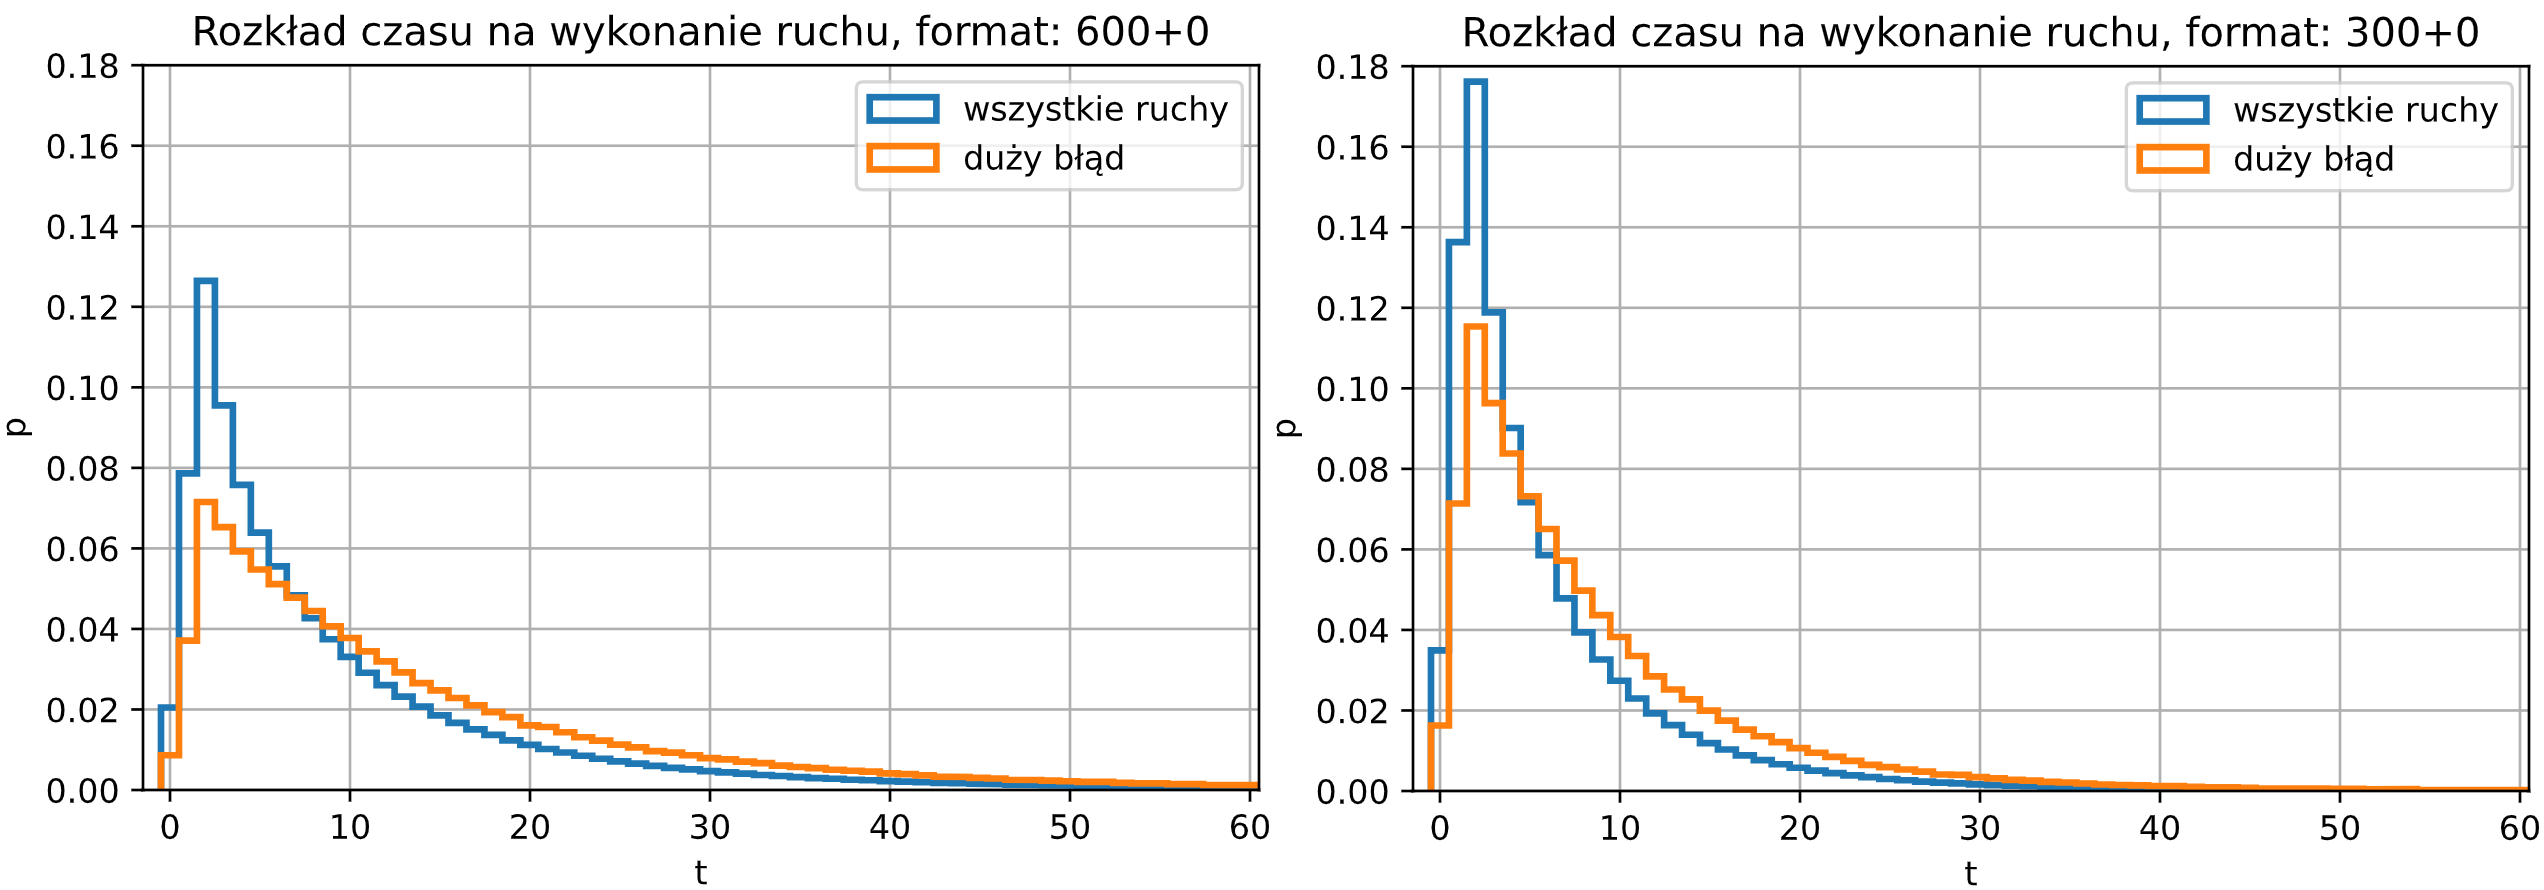
\includegraphics[width=\textwidth]{rozklad_czasu.png}
	\caption{
		blblalsdlasdlasldlad.}
	\label{rys:rozklad_czasu}
\end{figure}

\textbf{PLAN:}\\

\textbf{porównanie rozkładu czasu wykonania wszystkich ruchów oraz dla ruchów blunder (histogram gęstości)\\
	wskazanie różnicy\\
osobno rankingi przeanalizować}\\

\textbf{POMYSŁ! WZIĘCIE LOSOWE RUCHY Z ROZKŁADU TAKIEGO JAK ROZKŁAD RUCHÓW BLUNDER I SPRAWDZENIE RÓŻNICY MIĘDZY BLUNDER A LOSOWYMI RUCHAMI}


































Po przyjrzeniu się danym można zauważyć, że pochodzą one z rozkładu logarytmicznie-normalnego, co można uwarunkować tym, że w zdecydowanej większości pozycji zawodnik potrzebuje chwili na odpowiedź na ruch przeciwnika, tj 



TUTAJ rozkłady, 	

np dla formatu 60+0 (60 sekund, brak dodawanego czasu po wykonaniu ruchu)

\begin{figure}[H]
	\centering
	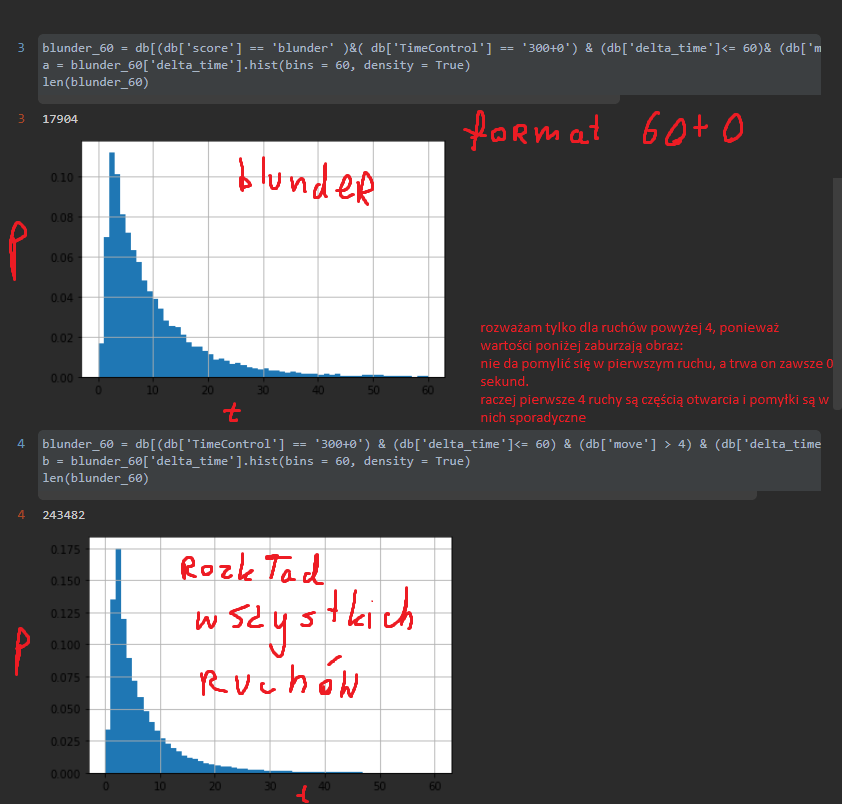
\includegraphics[width=\textwidth]{sample60.png}
	\caption{xxx}\label{xxx}
\end{figure}


oś x -> czas

oś y -> nieznormalizowana liczba ruchów typu 'blunder' (te najcięższe pomyłki)\newline


rozkład gamma... (?)\newline 




TO DO: 

sprawdzenie zmian dla rankingu graczy, różnicy rankingu graczy

porównanie z czasem na wykonanie każdego ruchu\newline



TO DO: 

czy różnica pomiędzy formatem z dodawanym czasem po ruchu, a bez dodawanego czasu jest widoczna?




tutaj statystyczne prawdopodobieństwo wykonania złego ruchu pod warunkiem poświęceniu mu konkretnego czasu,\newline

np, w formacie czasowym 60+0 na ruch zostały poświęcone 4 sekundy, jaka jest szansa, że został popełniony błąd \newline


CEL: 
ile powinno się poświęcić czasu na ruch by obniżyć prawdopodobieństwo wykonania błędu?\newline


\textbf{Tego jeszcze nie analizowałem}



w którym ruchu jest największa szansa na popełnienie błędu?
dla wszystkich rang
\begin{figure}[H]
	\centering
	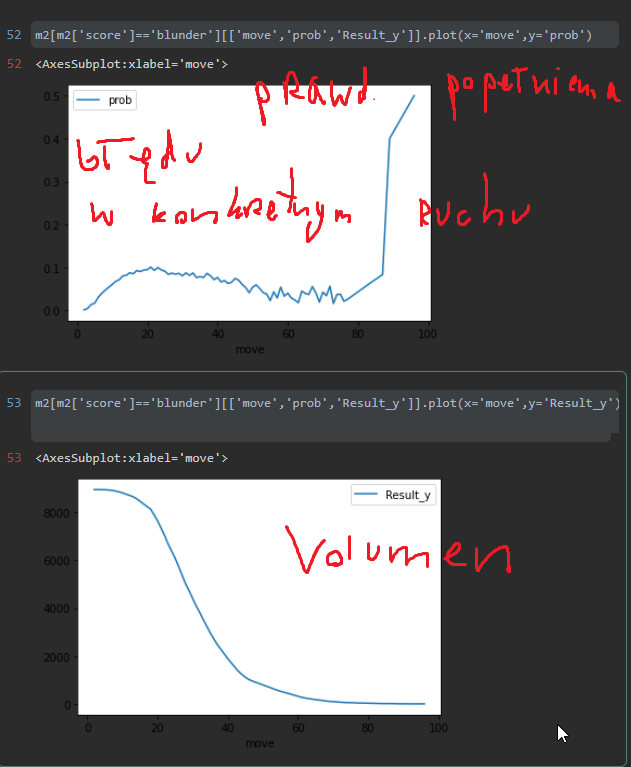
\includegraphics[width=\textwidth]{p_od_ruchu.png}
	\caption{aaa}\label{aaa}
\end{figure}

\chapter{wnioski, podsumowanie}
\begin{itemize}
	\item 95\% gier kończy się w 57 ruchach
	\item błąd dla każdego elo dla każdego posunięcia zajmuje średnio dłużej, ma też zawsze większą wariancje
	\item wszystkie ruchy: lepsi gracze szybciej wykonują ruchy początkowe, dłużej te z największą szansą na błąd (ok 20)
	\item największa szansa na błąd -- okolice 20 ruchu
	\item odnośnie dwóch poprzednich, lepsi gracze najmniej popełniają błędów w okolicach 20 ruchu
	\item największa szansa na błąd -- różnice dla elo (dużo błędów na początku 
	dla słabych graczy pozniej sie stabilizuje)
	\item lepsi gracze DŁUŻEJ wykonują ruchy BŁĘDNE
	\item różnice między formatami - w 600+0 ruchy zajmują nieliniowo więcej czasu, w 300+0 gracze są zmuszeni szybko wykonywać ruchy późniejsze.
	\item 10 pierwszych ruchów, istotna różnica w popełnieniu rażącego błędu między graczami słabymi a dobrymi
\end{itemize}


\chapter{tabelka}
Tabela \ref{tab:przykladowa} 
\begin{table}[H]
	\caption{Podstawowa Tabela}
	\centering
	\begin{tabular}{ccc}
		\hline
		\hline                       
		Państwo & PKB (w milionach USD )& Stopa bezrobocia  \\  [0.5ex] 
		\hline 
		Stany Zjednoczone & 75 278 049 & 4,60\%  \\
		Chiny & 11 218 281 & 4,10\%   \\
		Japonia & 4 938 644 & 3,10\%  \\
		Niemcy & 3 466 639 & 6,00\%   \\
		Wielka Brytania & 2 629 188 & 4,60\%  \\ [1ex]  
		\hline 
	\end{tabular}
	\caption*{\textit{Źródło: opracowanie własne}}
	\label{tab:przykladowa2} 
\end{table}

\chapter{Definicje, lematy, twierdzenia, przykłady i wnioski}
Definicje, lematy, twierdzenia, przykłady i wnioski piszemy w pracy tak:
\begin{definition}[Martyngał]
	Tu piszemy taratreść definicji martyngału.
\end{definition}
\begin{lemma}[]% w nawiasie kwadratowym można napisać jego nazwę
	Tu piszemy treść lematu.
\end{lemma}
\chapter{cytowanie}
Do cytowania używamy komendy \texttt{cite}. W nawiasie klamrowym podajemy klucz, którego użyliśmy w pliku \emph{bibliografia.bib}. Przykład: \cite{einstein} lub \cite[chap. 2]{latexcompanion}.

%{\backmatter \chapter{Podsumowanie}}
%Podsumowanie w pracach matematycznych nie jest obligatoryjne. Warto jednak na zakończenie krótko napisać, co udało nam się %zrobić w pracy, a czasem także o tym, czego nie udało się zrobić.



%%%%%%%%%%%%%%%%%%%%%%%%%%%%%%%%%%%%%%%%%%%%%%%%%%%%%%%%%
% BIBLIOGRAFIA
% W tworzeniu bibliografii najlepiej korzystać z BibTex'a, 
% który jest częścią systemu Tex. W naszym przypadku funkcję 
% przechowalni literatury, do której się odwołujemy, pełni 
% plik bibliografia.bib. Nie musimy ręcznie dodawać nowych 
% pozycji do bibliografii. Możemy wejść np. na stronę 
% https://mathscinet.ams.org/mathscinet/index.html, 
% znaleźć odpowiednią pozycję, wybrać ją, a następnie zmienić 
% 'Select alternative format' na BibTeX, skopiować uzyskany 
% tekst, wkleić do pliku bibliografia.bib i skompilować. 
% Gotowe informacje do pliku bibliografia.bib można znaleźć 
% także na https://arxiv.org - gdy znajdziemy interesującą nas 
% pracę, szukamy 'References & Citations' i klikamy 'NASA ADS', 
% a potem 'Bibtex entry for this abstract' 
% i postępujemy tak jak wcześniej.
%%%%%%%%%%%%%%%%%%%%%%%%%%%%%%%%%%%%%%%%%%%%%%%%%%%%%%%%%
\newpage
% w nawiasie klamrowym wpisujemy nazwę pliku z bibliografią w formacie .bib
\bibliography{bibliografia} 
\end{document}